%% LyX 2.3.7 created this file.  For more info, see http://www.lyx.org/.
%% Do not edit unless you really know what you are doing.
\documentclass[journal,article,submit,pdftex,moreauthors]{mdpi}
\usepackage[utf8]{inputenc}
\usepackage{float}
\usepackage{url}
\usepackage{amsmath}
\usepackage{graphicx}

\makeatletter

%%%%%%%%%%%%%%%%%%%%%%%%%%%%%% LyX specific LaTeX commands.

\Title{Using optimization techniques in Grammatical Evolution}

\TitleCitation{Using optimization techniques in Grammatical Evolution}

\Author{Ioannis G. Tsoulos$^{1,*}$, Alexandros Tzallas$^{2}$, Evangelos
Karvounis$^{3}$}

\AuthorNames{Ioannis G. Tsoulos; Alexandros Tzallas;Evangelos Karvounis}

\AuthorCitation{Tsoulos, I.G.; Tzallas A; Karvounis E;}


\address{$^{1}$\quad{}Department of Informatics and Telecommunications,
University of Ioannina, Greece;itsoulos@uoi.gr\\
$^{2}\quad$Department of Informatics and Telecommunications, University
of Ioannina, Greece;tzallas@uoi.gr\\
$^{3}\quad$Department of Informatics and Telecommunications, University
of Ioannina, Greece;ekarvounis@uoi.gr}


\corres{Correspondence: itsoulos@uoi.gr; }


\abstract{The Grammatical Evolution technique has been successfully applied
to a wide range of problems in various scientific fields. However,
in many cases, techniques that make use of Grammatical Evolution get
trapped in local minima of the objective problem and fail to reach
the optimal solution. One simple method to tackle such situations
is the usage of hybrid techniques, where local minimization algorithms
are used in conjunction with the main algorithm. However, Grammatical
Evolution is an integer optimization problem and, as a consequence,
techniques should be formulated that are applicable to it as well.
In current work, a modified version of the Simulated Annealing algorithm
is used as a local optimization procedure in Grammatical Evolution.
This approach was tested on the Constructed Neural Networks and a
remarkable improvement of the experimental results was shown, both
in classification data and in data fitting cases.\textbf{ }}


\keyword{Grammatical Evolution; Optimization techniques; Neural networks;
Evolutionary techniques; Stochastic methods.}

\DeclareTextSymbolDefault{\textquotedbl}{T1}
%% Because html converters don't know tabularnewline
\providecommand{\tabularnewline}{\\}
\floatstyle{ruled}
\newfloat{algorithm}{tbp}{loa}
\providecommand{\algorithmname}{Algorithm}
\floatname{algorithm}{\protect\algorithmname}

%%%%%%%%%%%%%%%%%%%%%%%%%%%%%% Textclass specific LaTeX commands.
\newenvironment{lyxcode}
	{\par\begin{list}{}{
		\setlength{\rightmargin}{\leftmargin}
		\setlength{\listparindent}{0pt}% needed for AMS classes
		\raggedright
		\setlength{\itemsep}{0pt}
		\setlength{\parsep}{0pt}
		\normalfont\ttfamily}%
	 \item[]}
	{\end{list}}

%%%%%%%%%%%%%%%%%%%%%%%%%%%%%% User specified LaTeX commands.
%  LaTeX support: latex@mdpi.com 
%  For support, please attach all files needed for compiling as well as the log file, and specify your operating system, LaTeX version, and LaTeX editor.

%=================================================================


% For posting an early version of this manuscript as a preprint, you may use "preprints" as the journal and change "submit" to "accept". The document class line would be, e.g., \documentclass[preprints,article,accept,moreauthors,pdftex]{mdpi}. This is especially recommended for submission to arXiv, where line numbers should be removed before posting. For preprints.org, the editorial staff will make this change immediately prior to posting.

%--------------------
% Class Options:
%--------------------
%----------
% journal
%----------
% Choose between the following MDPI journals:
% acoustics, actuators, addictions, admsci, adolescents, aerospace, agriculture, agriengineering, agronomy, ai, algorithms, allergies, alloys, analytica, animals, antibiotics, antibodies, antioxidants, applbiosci, appliedchem, appliedmath, applmech, applmicrobiol, applnano, applsci, aquacj, architecture, arts, asc, asi, astronomy, atmosphere, atoms, audiolres, automation, axioms, bacteria, batteries, bdcc, behavsci, beverages, biochem, bioengineering, biologics, biology, biomass, biomechanics, biomed, biomedicines, biomedinformatics, biomimetics, biomolecules, biophysica, biosensors, biotech, birds, bloods, blsf, brainsci, breath, buildings, businesses, cancers, carbon, cardiogenetics, catalysts, cells, ceramics, challenges, chemengineering, chemistry, chemosensors, chemproc, children, chips, cimb, civileng, cleantechnol, climate, clinpract, clockssleep, cmd, coasts, coatings, colloids, colorants, commodities, compounds, computation, computers, condensedmatter, conservation, constrmater, cosmetics, covid, crops, cryptography, crystals, csmf, ctn, curroncol, currophthalmol, cyber, dairy, data, dentistry, dermato, dermatopathology, designs, diabetology, diagnostics, dietetics, digital, disabilities, diseases, diversity, dna, drones, dynamics, earth, ebj, ecologies, econometrics, economies, education, ejihpe, electricity, electrochem, electronicmat, electronics, encyclopedia, endocrines, energies, eng, engproc, ent, entomology, entropy, environments, environsciproc, epidemiologia, epigenomes, est, fermentation, fibers, fintech, fire, fishes, fluids, foods, forecasting, forensicsci, forests, foundations, fractalfract, fuels, futureinternet, futureparasites, futurepharmacol, futurephys, futuretransp, galaxies, games, gases, gastroent, gastrointestdisord, gels, genealogy, genes, geographies, geohazards, geomatics, geosciences, geotechnics, geriatrics, hazardousmatters, healthcare, hearts, hemato, heritage, highthroughput, histories, horticulturae, humanities, humans, hydrobiology, hydrogen, hydrology, hygiene, idr, ijerph, ijfs, ijgi, ijms, ijns, ijtm, ijtpp, immuno, informatics, information, infrastructures, inorganics, insects, instruments, inventions, iot, j, jal, jcdd, jcm, jcp, jcs, jdb, jeta, jfb, jfmk, jimaging, jintelligence, jlpea, jmmp, jmp, jmse, jne, jnt, jof, joitmc, jor, journalmedia, jox, jpm, jrfm, jsan, jtaer, jzbg, kidney, kidneydial, knowledge, land, languages, laws, life, liquids, literature, livers, logics, logistics, lubricants, lymphatics, machines, macromol, magnetism, magnetochemistry, make, marinedrugs, materials, materproc, mathematics, mca, measurements, medicina, medicines, medsci, membranes, merits, metabolites, metals, meteorology, methane, metrology, micro, microarrays, microbiolres, micromachines, microorganisms, microplastics, minerals, mining, modelling, molbank, molecules, mps, msf, mti, muscles, nanoenergyadv, nanomanufacturing, nanomaterials, ncrna, network, neuroglia, neurolint, neurosci, nitrogen, notspecified, nri, nursrep, nutraceuticals, nutrients, obesities, oceans, ohbm, onco, oncopathology, optics, oral, organics, organoids, osteology, oxygen, parasites, parasitologia, particles, pathogens, pathophysiology, pediatrrep, pharmaceuticals, pharmaceutics, pharmacoepidemiology, pharmacy, philosophies, photochem, photonics, phycology, physchem, physics, physiologia, plants, plasma, pollutants, polymers, polysaccharides, poultry, powders, preprints, proceedings, processes, prosthesis, proteomes, psf, psych, psychiatryint, psychoactives, publications, quantumrep, quaternary, qubs, radiation, reactions, recycling, regeneration, religions, remotesensing, reports, reprodmed, resources, rheumato, risks, robotics, ruminants, safety, sci, scipharm, seeds, sensors, separations, sexes, signals, sinusitis, skins, smartcities, sna, societies, socsci, software, soilsystems, solar, solids, sports, standards, stats, stresses, surfaces, surgeries, suschem, sustainability, symmetry, synbio, systems, taxonomy, technologies, telecom, test, textiles, thalassrep, thermo, tomography, tourismhosp, toxics, toxins, transplantology, transportation, traumacare, traumas, tropicalmed, universe, urbansci, uro, vaccines, vehicles, venereology, vetsci, vibration, viruses, vision, waste, water, wem, wevj, wind, women, world, youth, zoonoticdis 

%---------
% article
%---------
% The default type of manuscript is "article", but can be replaced by: 
% abstract, addendum, article, book, bookreview, briefreport, casereport, comment, commentary, communication, conferenceproceedings, correction, conferencereport, entry, expressionofconcern, extendedabstract, datadescriptor, editorial, essay, erratum, hypothesis, interestingimage, obituary, opinion, projectreport, reply, retraction, review, perspective, protocol, shortnote, studyprotocol, systematicreview, supfile, technicalnote, viewpoint, guidelines, registeredreport, tutorial
% supfile = supplementary materials

%----------
% submit
%----------
% The class option "submit" will be changed to "accept" by the Editorial Office when the paper is accepted. This will only make changes to the frontpage (e.g., the logo of the journal will get visible), the headings, and the copyright information. Also, line numbering will be removed. Journal info and pagination for accepted papers will also be assigned by the Editorial Office.

%------------------
% moreauthors
%------------------
% If there is only one author the class option oneauthor should be used. Otherwise use the class option moreauthors.

%---------
% pdftex
%---------
% The option pdftex is for use with pdfLaTeX. If eps figures are used, remove the option pdftex and use LaTeX and dvi2pdf.

%=================================================================
% MDPI internal commands
\firstpage{1} 
 
\setcounter{page}{\@firstpage} 

\pubvolume{1}
\issuenum{1}
\articlenumber{0}
\pubyear{2022}
\copyrightyear{2022}
%\externaleditor{Academic Editor: Firstname Lastname} % For journal Automation, please change Academic Editor to "Communicated by"
\datereceived{} 
\dateaccepted{} 
\datepublished{} 
%\datecorrected{} % Corrected papers include a "Corrected: XXX" date in the original paper.
%\dateretracted{} % Corrected papers include a "Retracted: XXX" date in the original paper.
\hreflink{https://doi.org/} % If needed use \linebreak
%\doinum{}
%------------------------------------------------------------------
% The following line should be uncommented if the LaTeX file is uploaded to arXiv.org
%\pdfoutput=1

%=================================================================
% Add packages and commands here. The following packages are loaded in our class file: fontenc, inputenc, calc, indentfirst, fancyhdr, graphicx, epstopdf, lastpage, ifthen, lineno, float, amsmath, setspace, enumitem, mathpazo, booktabs, titlesec, etoolbox, tabto, xcolor, soul, multirow, microtype, tikz, totcount, changepage, attrib, upgreek, cleveref, amsthm, hyphenat, natbib, hyperref, footmisc, url, geometry, newfloat, caption

%=================================================================
%% Please use the following mathematics environments: Theorem, Lemma, Corollary, Proposition, Characterization, Property, Problem, Example, ExamplesandDefinitions, Hypothesis, Remark, Definition, Notation, Assumption
%% For proofs, please use the proof environment (the amsthm package is loaded by the MDPI class).

%=================================================================
% The fields PACS, MSC, and JEL may be left empty or commented out if not applicable
%\PACS{J0101}
%\MSC{}
%\JEL{}

%%%%%%%%%%%%%%%%%%%%%%%%%%%%%%%%%%%%%%%%%%
% Only for the journal Diversity
%\LSID{\url{http://}}

%%%%%%%%%%%%%%%%%%%%%%%%%%%%%%%%%%%%%%%%%%
% Only for the journal Applied Sciences:
%\featuredapplication{Authors are encouraged to provide a concise description of the specific application or a potential application of the work. This section is not mandatory.}
%%%%%%%%%%%%%%%%%%%%%%%%%%%%%%%%%%%%%%%%%%

%%%%%%%%%%%%%%%%%%%%%%%%%%%%%%%%%%%%%%%%%%
% Only for the journal Data:
%\dataset{DOI number or link to the deposited data set in cases where the data set is published or set to be published separately. If the data set is submitted and will be published as a supplement to this paper in the journal Data, this field will be filled by the editors of the journal. In this case, please make sure to submit the data set as a supplement when entering your manuscript into our manuscript editorial system.}

%\datasetlicense{license under which the data set is made available (CC0, CC-BY, CC-BY-SA, CC-BY-NC, etc.)}

%%%%%%%%%%%%%%%%%%%%%%%%%%%%%%%%%%%%%%%%%%
% Only for the journal Toxins
%\keycontribution{The breakthroughs or highlights of the manuscript. Authors can write one or two sentences to describe the most important part of the paper.}

%%%%%%%%%%%%%%%%%%%%%%%%%%%%%%%%%%%%%%%%%%
% Only for the journal Encyclopedia
%\encyclopediadef{Instead of the abstract}
%\entrylink{The Link to this entry published on the encyclopedia platform.}
%%%%%%%%%%%%%%%%%%%%%%%%%%%%%%%%%%%%%%%%%%

\makeatother

\begin{document}
\maketitle

\section{Introduction}

Genetic Algorithms belong to the field of evolutionary techniques
\citep{ec_review} and were originally formulated by John Hollands
and his team \citep{Holland1}. Genetic Algorithms are initiated by
generating a series of random candidate solutions to an optimization
problem. These candidate solutions are called chromosomes, and they
iteratively undergo a series of operations that have their foundation
in physical processes, such as selection, crossover, and mutation
\citep{Stender,genetic1,genetic2}. Grammatical Evolution \citep{ge1}
is considered as a special case of genetic algorithms, where the chromosomes
are series of integer numbers.\textbf{ }Chromosomes in the Grammatical
Evolution process are rules for generating a BNF grammar \citep{bnf1}
and can be used to create functional programs in any programming language. 

Grammatical Evolution has been applied on a wide series of real -
world applications, such as\textbf{ }function approximation\citep{ge_program1,ge_program2},
credit classification \citep{ge_credit}, network security and prevention
of attacks \citep{ge_intrusion}, monitoring of water quality \citep{ge_water},
modeling glycemia in humans \citep{ge_glykemia}, automatic design
of Ant algorithms \citep{ge_ant},\textbf{ }temperature prediction
in data centers \citep{ge_datacenter},\textbf{ }solving trigonometric
equations \citep{ge_trig},\textbf{ }composing music \citep{ge_music},\textbf{
}neural network construction \citep{ge_nn,ge_nn2},\textbf{ }producing
numeric constants \citep{ge_constant},\textbf{ }video games \citep{ge_pacman,ge_supermario},\textbf{
}energy demand estimation\citep{ge_energy},\textbf{ }combinatorial
optimization \citep{ge_comb}, cryptography \citep{ge_crypt}, evolving
of decision trees \citep{ge_decision},\textbf{ }automatic design
of analog electronic circuits \citep{ge_analog} etc.

The method of Grammatical Evolution has been extended by various researchers
during the last years and some examples of these extensions are the\textbf{
}Structured Grammatical Evolution \citep{ge_structured1,ge_structured2},\textbf{
}that applies an one-to-one mapping between the chromosomes and the
non-terminal symbols of the grammar,\textbf{ }the $\pi$Grammatical
Evolution method \citep{pge}, application of the Particle Swarm Optimization(PSO)
\citep{pso1} to produce programs with grammatical evolution denoted
as Grammatical Swarm \citep{ge_swarm1,ge_swarm2},\textbf{ }the Probabilistic
Grammatical Evolution \citep{probge} which introduced a new mapping
mechanism for the Grammatical Evolution method,\textbf{ }incorporation
of parallel programming techniques \citep{ge_par1,ge_par2}, usage
of Christiansen grammars \citep{ge_christiansen} etc. 

Also, a variety of software has been developed for Grammatical Evolution,
such as the GEVA \citep{ge_geva} that proposes a GUI application
for Grammatical Evolution, the gramEvol software \citep{ge_gramevol}
that provides a package in the R programming language, the GeLab \citep{ge_gelab}
that implements a Matlab toolbox for Grammatical Evolution, the GenClass
\citep{ge_genclass} software used to produce classification programs,
the QFc software \citep{ge_qfc} for feature construction etc.

Although the method of Grammatical Evolution has proven to be extremely
efficient, it can often get trapped in local minimum of the objective
problem and its performance may not be as expected. A common method
to get out of such situations is the use of local optimization techniques,
which have been applied many times in combination with Genetic Algorithms
\citep{ge_local1,ge_local2}. In the case of Grammatical Evolution
and due to the integral representation of the candidate solutions,
local optimization techniques are not directly applicable, such as,
for example, the BFGS method \citep{bfgs} and hence more suitable
methods should be adopted.\textbf{ }In this paper, an attempt is made
to improve upon the excellent results shown by Grammatical Evolution
in the past on a variety of problems by applying local optimization
techniques, periodically applied to randomly selected chromosomes
of Grammatical Evolution. The current work utilizes a modified version
of the Simulated Annealing method \citep{siman_main} as a local search
procedure. The method of Simulated Annealing has been utilized in
various cases, such as image processing \citep{siman_image}, protein
structure optimization \citep{siman_protein}, resource allocation
\citep{siman_resource}, convex optimization \citep{siman_convex},
deep learning \citep{siman_deep} etc. To verify the possibility of
the proposed methodology to improve the results of Grammatical Evolution,
the Neural Networks construction technique was chosen. This method
was initally provided in \citep{nnc_tsoulos} and it can estimate
the topology and the weights of neural networks using the Grammatical
Evolution procedure. This method was chosen to test the present methodology
because of its many applications. However, the technique proposed
in this paper will be able to be applied in the future in other cases
of using Grammatical Evolution. To evaluate the performance of the
modified technique it was evaluated on a extended series of classification
and regression problems found in the relevant literature and the results
seem to be promising.

This paper has the following sections: section \ref{sec:The-proposed-method}
the Grammatical Evolution procedure is discussed and the proposed
modification is described, the section \ref{sec:Results} presents
the datasets used in the experiments as well as the results from the
conducted experimentsand finally the section \ref{sec:Conclusions}
provides some conclusions and guidelines for future work.

\section{The proposed method\label{sec:The-proposed-method}}

This section starts with a brief description of the Grammatical Evolution
process and the grammar used, then the modified Simulated Annealing
method is presented, and finally the artificial neural network construction
algorithm will be presented. 

\subsection{The Grammatical Evolution method \label{subsec:The-Grammatical-Evolution}}

The chromosomes of Grammatical Evolution stand for production rules
of the given BNF grammar. BNF grammars are usually defined as a tuple
\textbf{$G=\left(N,T,S,P\right)$}, where
\begin{itemize}
\item \textbf{$N$ }is the set of non-terminal symbols.
\item \textbf{$T$ }is the set of terminal symbols.\textbf{ }
\item $S$ represents that start symbol of the grammar with $S\in N$.
\item \textbf{$P$ }is the production rules of the grammar. Usually these
rules are in the form \textbf{$A\rightarrow a$ }or\textbf{ $A\rightarrow aB,\ A,B\in N,\ a\in T$.}
\end{itemize}
The BNF grammar is extended by using enumeration in the the production
rules. The grammar shown in Figure \ref{fig:BNF-grammar-of} is used
to construct artificial neural networks expressed in the form:
\begin{equation}
N\left(\overrightarrow{x},\overrightarrow{w}\right)=\sum_{i=1}^{H}w_{(d+2)i-(d+1)}\sigma\left(\sum_{j=1}^{d}x_{j}w_{(d+2)i-(d+1)+j}+w_{(d+2)i}\right)\label{eq:nn}
\end{equation}
where the parameter $H$ represents the number of processing units
(hidden noes) for the neural network and the value $d$ represents
the of the vector $\overrightarrow{x}.$ Also, the vector $\overrightarrow{w}$
represents the vector of parameters for the neural network. The function
sig(x) represents the sigmoid function $\sigma(x)$ defined as: 
\begin{equation}
\sigma(x)=\frac{1}{1+\exp(-x)}\label{eq:sig}
\end{equation}

The notation \textless\textgreater{} is used for the non - terminal
symbols of the grammar. The sequence numbers of the production rules
are inside the parentheses of the extended grammar. The constant d
stands for the dimension of the provided dataset. The production of
valid expressions initiates from the symbol $S$ and using a series
of steps, creates a program by replacing non - terminal symbols with
the right hand of the selected production rule. The Grammatical Evolution
selects production rules using the following scheme:
\begin{itemize}
\item Obtain the next element V from the provided chromosome.
\item The production rule is selected according to the scheme 
\begin{equation}
\mbox{Rule} =V\ \mbox{mod}\ \mbox{NR}
\end{equation}
where NR is the total number of production rules for the current non
-- terminal symbol. 
\end{itemize}
\begin{figure}
\caption{The used grammar in Neural Network Construction.\label{fig:BNF-grammar-of}}

\begin{lyxcode}
S:=\textless sigexpr\textgreater ~~~~~~~~~~~~~~~~~~~~~~~~~~(0)

\textless sigexpr\textgreater ::=\textless Node\textgreater ~~~~~~~~~~~~~~~~~~~~(0)

~~~~~~~~~~~\textbar ~\textless Node\textgreater ~+~\textless sigexpr\textgreater ~~~~~~~(1)

\textless Node\textgreater ::=\textless number\textgreater{*}sig(\textless sum\textgreater +\textless number\textgreater )~(0)

\textless sum\textgreater ::=~\textless number\textgreater{*}\textless xxlist\textgreater ~~~~~~~~~~~~(0)

~~~~~~~~~~~\textbar ~~~~\textless sum\textgreater +\textless sum\textgreater ~~~~~~~~~~~(1)

\textless xxlist\textgreater ::=~x1~~~~~~~~(0)

~~~~~~~~~~~~~\textbar ~~~~x2~~(1)

~~~~~~~~~~~~~..............

~~~~~~~~~~~~~\textbar ~~~~xd~~(d-1)

\textless number\textgreater ::=~(\textless digitlist\textgreater .\textless digitlist\textgreater )~~~~~~~~(0)

~~~~~~~~~~~~~\textbar ~~~~(-\textless digitlist\textgreater .\textless digitlist\textgreater )~(1)

\textless digitlist\textgreater ::=~\textless digit\textgreater ~~~~~~~~~~~~(0)

~~~~~~~~~~~~~\textbar ~\textless digit\textgreater\textless digitlist\textgreater ~(1)

\textless digit\textgreater ::=~0~~~~~~(0)

~~~~~~~~~~~~~\textbar ~~1~(1)

~~~~~~~~~~~~~...........

~~~~~~~~~~~~~\textbar ~~9~(9)
\end{lyxcode}
\end{figure}


\subsection{The modified Simulated Annealing algorithm}

The current work utilizes a modified version of the Simulated Annealing
algorithm as a local search procedure. The main steps of this procedure
are shown in Algorithm \ref{alg:siman}.

\begin{algorithm}[H]
\caption{The modified version of the Simulated Annealing algorithm.\label{alg:siman}}

\textbf{procedure} siman$\left(x_{0}\right)$
\begin{enumerate}
\item \textbf{Set} $k=0$, $T_{0}>0,\ \epsilon>0,$$r_{T}>0,\ r_{T}<1$..
\item \textbf{Set} $N_{eps}>0$, a positive integer indicated the number
of samples drawn in every iteration.
\item \textbf{Set }$g$ and $R$, positive integer values.
\item \textbf{Set} $x_{b}=x_{0},f_{b}=f\left(x_{b}\right)$.
\item \textbf{For} $i=1\ldots N_{\mbox{eps}}$ \label{enu:For-}

\begin{enumerate}
\item \textbf{Set} $y=x_{k}$
\item \textbf{For} $j=1\ldots g$
\begin{enumerate}
\item \textbf{Set} $p=\mbox{rand}\left(1,\mbox{size}\left(x_{0}\right)\right)$.
The variable $p$ indicates a randomly selected position in $y$.
\item \textbf{Set} $y_{p}=y_{p}+\mbox{rand}\left(-R,R\right)$
\end{enumerate}
\item \textbf{EndFor}
\item \textbf{If $f(y)\le f\left(x_{k}\right)$ then $x_{k+1}=y$}
\item \textbf{Else Set} $x_{k+1}=y$ with probability $\min\left\{ 1,\exp\left(-\frac{f(y)-f\left(x_{k}\right)}{T_{k}}\right)\right\} $
\item \textbf{If} $f\left(y\right)<f_{b}$ \textbf{then} $x_{b}=y,f_{b}=f(y)$.
\end{enumerate}
\item \textbf{EndFor}
\item \textbf{Set} $T_{k+1}=T_{k}r_{T}$
\item \textbf{Set} $k=k+1$.
\item If $T_{k}\le\epsilon$ terminate
\item \textbf{Goto} step \ref{enu:For-}.
\item \textbf{Return }$x_{b}$
\end{enumerate}
\textbf{end} siman
\end{algorithm}
The method accepts the chromosome $x_{0}$ as a starting point and,
in each iteration, randomly generates chromosomes around it. The parameter
$g$ controls the number of changes that will be made to the chromosome
and the parameter $R$ controls the radius of these changes. The parameter
$T$ represents the temperature of the algorithm. The temperature
starts at extremely high values and progressively decreases linearly.
In the early stages and at high temperatures the algorithm may accept
points that may have higher values of the fitness function, but as
the temperature decreases, this probability also decreases. 

\subsection{The Neural Network Construction algorithm}

The main steps of the algorithm used to construct artificial neural
networks with Grammatical Evolution are listed below:
\begin{enumerate}
\item \textbf{Initialization} step.
\begin{enumerate}
\item \textbf{Set} $N_{g}$ as the maximum number of generations allowed.
\item \textbf{Set} $N_{c}$ as the number of chromosomes. 
\item \textbf{Set} $p_{s}$ as the selection rate and $p_{m}$ as the mutation
rate. 
\item \textbf{Define} as $L_{i}$ the number of generations that should
elapse before applying the local optimization technique.
\item \textbf{Define} as $L_{c}$ the number of chromosomes involved in
the local search procedure.
\item \textbf{Initialize} the chromosomes. Each chromosome is considered
as a series of randomly initialized integers.
\item \textbf{Set} iter=0
\end{enumerate}
\item \textbf{Genetic} step
\begin{enumerate}
\item \textbf{For} $i=1,\ldots,N_{g}$ \textbf{do}
\begin{enumerate}
\item \textbf{Create} for every chromosome a neural network $C_{i}$ using
the Grammatical Evolution procedure of subsection \ref{subsec:The-Grammatical-Evolution}
and the associated grammar given in Figure \ref{fig:BNF-grammar-of}.
\item \textbf{Calculate} the fitness $f_{i}$ on the train set of the objective
problem as:
\begin{equation}
f_{i}=\sum_{j=1}^{M}\left(C_{i}\left(\overrightarrow{x}_{j}\right)-t_{j}\right)^{2}\label{eq:eq1}
\end{equation}
where the set $\left(\overrightarrow{x_{j}},t_{j}\right),\ j=1,...,M$
is train dataset, with $t_{i}$ being the actual output for the point
$\overrightarrow{x_{i}}$ . 
\item \textbf{Perform} the selection procedure. Initially, the chromosomes
are sorted according to their fitness values. The best\textbf{ $\left(1-p_{s}\right)\times N_{c}$}
chromosomes are transferred to the next generation.\textbf{ }The remaining
chromosomes will be replaced by offsprings created during the crossover
procedure. 
\item \textbf{Perform} the crossover procedure. The crossover procedure
produces $p_{s}\times N_{c}$ offsprings. For every pair of produced
offsprings $\tilde{z}$ and $\tilde{w}$, two offsprings $(z,w)$.
The selection is performed using tournament selection. The new offsprings
are produced using the one - point crossover procedure. An example
of the one - point crossover procedure is shown in Figure \ref{fig:onePoint}.
\item \textbf{Perform} the mutation procedure. For each element of every
chromosome, a random number $r\in\left[0,1\right]$ is drawn. The
corresponding element is altered if $r\le p_{m}$.
\end{enumerate}
\item \textbf{EndFor} 
\end{enumerate}
\item \textbf{Local Search Step }

\begin{enumerate}
\item \textbf{If }$\mbox{iters}\ \mod\ L_{i}=0$ \textbf{Then}

\begin{enumerate}
\item \textbf{Create }a set of randomly $L_{C}$ chosen chromosomes from
the genetic population. Denote this set as $L_{S}$ .
\item \textbf{For} every $X_{k}$ \textbf{in} $L_{S}$ apply the modified
Simulated Annealing algorithm given in Algorithm \ref{alg:siman}:
$X_{k}=\mbox{siman}\left(X_{k}\right)$
\end{enumerate}
\end{enumerate}
\item \textbf{set} iter=iter+1. \textbf{If} iter$>$$N_{g}$ \textbf{goto}
Evaluation step else \textbf{goto} Genetic step.
\item \textbf{Evaluation} step
\begin{enumerate}
\item Get the chromosome with the lowest fitness value and create the associated
neural network $C^{*}$.
\item Evaluate the neural network $C^{*}$ in the test set of the underlying
dataset and report the results.
\end{enumerate}
\begin{figure}[H]
\begin{centering}
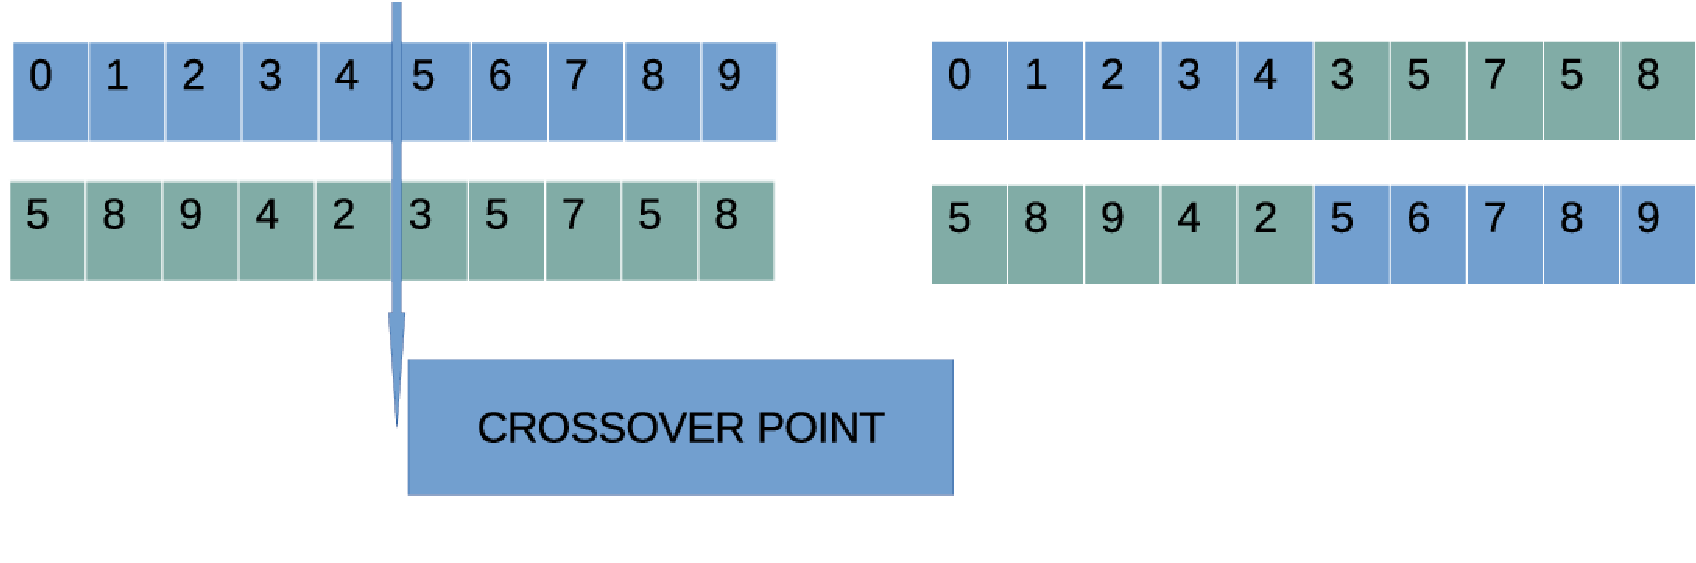
\includegraphics[scale=0.5]{onepoint_crossover}
\par\end{centering}
\caption{An example of the one - point crossover method, used in the Grammatical
Evolution procedure.\label{fig:onePoint}}

\end{figure}

\end{enumerate}

\section{Results\label{sec:Results}}

The current work was evaluated by executing a series of experiments
on some classification and regression datasets, commonly used in the
relevant literature. The obtained results were compared with other
machine learning techniques. These datasets can be downloaded freely
from the following websites:
\begin{enumerate}
\item The UCI dataset repository, \url{https://archive.ics.uci.edu/ml/index.php}(accessed
on 20 March 2024)\citep{UCL}
\item The Keel repository, \url{https://sci2s.ugr.es/keel/datasets.php}(accessed
on 20 March 2024)\citep{Keel}.
\item The Statlib URL \url{http://lib.stat.cmu.edu/datasets/ }(accessed
on 20 March 2024). 
\end{enumerate}

\subsection{Classification datasets }

The following series of classification datasets was used in the conducted
experiments:
\begin{enumerate}
\item \textbf{Appendictis} a medical dataset, provided in \citep{appendicitis}. 
\item \textbf{Australian} dataset \citep{australian}, which is related
to credit card transactions.
\item \textbf{Balance} dataset \citep{balance}, a dataset related to psychological
experiments.
\item \textbf{Circular} dataset, an artificial dataset that contains 1000
examples.
\item \textbf{Cleveland} dataset, a medical dataset used in a series of
papers \citep{cleveland1,cleveland2}.
\item \textbf{Dermatology} dataset \citep{dermatology}, which is a medical
dataset about dermatological deceases. 
\item \textbf{Ecoli} dataset, a dataset about protein localization sites
\citep{ecoli}.
\item \textbf{Haberman} dataset, related to breast cancer.
\item \textbf{Heart} dataset \citep{heart}, a medical dataset about heart
diseases.
\item \textbf{Hayes roth} dataset \citep{hayesroth}, which is a human subjects
study.
\item \textbf{HouseVotes} dataset \citep{housevotes}, related to votes
collected from U.S. House of Representatives Congressmen. 
\item \textbf{Ionosphere} dataset, that was used in experiments related
to the ionosphere \citep{ion1,ion2}.
\item \textbf{Liverdisorder} dataset \citep{liver}, a medical dataset related
to liver disorders.
\item \textbf{Mammographic} dataset \citep{mammographic}, a medical dataset
related to breast cancer.
\item \textbf{Parkinsons} dataset, a medical dataset related to the Parkinson's
disease (PD)\citep{parkinsons}.
\item \textbf{Pima} dataset \citep{pima}, a medical dataset related to
the diabetes presence.
\item \textbf{Popfailures} dataset \citep{popfailures}, a dataset related
to climate measurements.
\item \textbf{Regions2} dataset, medical dataset related to hepatitis C
\citep{regions}. 
\item \textbf{Saheart} dataset \citep{saheart}. This dataset is used to
detect heart diseases.
\item \textbf{Segment} dataset \citep{segment}, related to image processing.
\item \textbf{Student} dataset \citep{student}, related to data collected
in Portuguese schools. 
\item \textbf{Transfusion} dataset\citep{transfusion}, this datasets was
taken from the Blood Transfusion Service Center in Hsin-Chu City in
Taiwan.
\item \textbf{Wdbc} dataset \citep{wdbc}, a medical dataset related cancer
detection.
\item \textbf{Wine} dataset. This is a dataset used to detect the quality
of a series of wines. \citep{wine1,wine2}.
\item \textbf{Eeg} datasets, a dataset related to EEG measurements \citep{eeg}.
From this dataset the following cases were used: Z\_F\_S, Z\_O\_N\_F\_S,
ZO\_NF\_S and ZONF\_S.
\item \textbf{Zoo} dataset \citep{zoo}, related to animal classification.
\end{enumerate}

\subsection{Regression datasets }

The following regression datasets were used in the conducted experiments:
\begin{enumerate}
\item \textbf{Abalone} dataset \citep{abalone}, a dataset related to the
prediction of age of abalones.
\item \textbf{Airfoil }dataset, a dataset proposed by NASA \citep{airfoil}.
\item \textbf{Baseball} dataset, related with the income of baseball players. 
\item \textbf{Concrete} dataset \citep{concrete}, which is a civil engineering
dataset.
\item \textbf{Dee} dataset. This dataset has measures from the price of
electricity.
\item \textbf{HO} dataset, downloaded from the STALIB repository.
\item \textbf{Housing} dataset, mentioned in \citep{key23}.
\item \textbf{Laser} dataset.This is a dataset related to laser experiments
\item \textbf{LW} dataset, related to risk factors associated with low weight
babies.
\item \textbf{MORTGAGE} dataset, a dataset related to economic measurements
from USA.
\item \textbf{PL} dataset, provided from the STALIB repository.
\item \textbf{SN} dataset, provided from the STALIB repository.
\item \textbf{Treasury} dataset, a dataset related to economic measurements
from USA.
\item \textbf{TZ} dataset, provided from the STALIB repository.
\end{enumerate}

\subsection{Experimental results}

For the execution of the experiments, code written in ANSI C++ was
used and, with the help of the programming environment Optimus. The
software is freely available from \url{https://github.com/itsoulos/OPTIMUS/}(
accessed on 20 March 2024 ). The experiments were conducted 30 times.
In every execution different seed was used for the random number generator
and the function drand48() of the C programming language was used.
The validation of the results was performed using the technique of
10 - fold cross validation. The average classification error is reported
for the case of classification datasets and the average regression
error for the case of regression datasets. These errors are measured
on the corresponding test set. The values for the experimental parameters
are displayed in Table \ref{tab:experValues}. The experimental results
for the classification datasets are outlined in the table \ref{tab:tableClass}
and the results for the regression datasets are shown in the table
\ref{tab:tabRegression}. The following applies to the tables with
the experimental results:
\begin{enumerate}
\item The column DATASET denotes the used dataset.
\item The column ADAM denotes the application of the ADAM optimization method
\citep{Adam} in an artificial neural network with $H=10$ processing
nodes.
\item The column NEAT stands for the usage of NEAT method (NeuroEvolution
of Augmenting Topologies ) \citep{neat}.
\item The column MLP stands for the experimental results of an artificial
neural network with $H=10$ processing nodes. The neural network was
trained using a genetic algorithm and the BFGS local optimization
method \citep{powell}. 
\item The column RBF represents the application of an RBF network with $H=10$
processing nodes in each dataset.
\item The column NNC denotes the usage of the original Neural Construction
technique, that was constructed with Grammatical Evolution.
\item The column NNC-S denotes the usage of the proposed local optimization
procedure in the Neural Construction technique.
\item The line AVERAGE denotes the average classification or regression
error.
\end{enumerate}
\begin{table}[H]
\begin{centering}
\begin{tabular}{|c|c|c|}
\hline 
NAME & PURPOSE & VALUE\tabularnewline
\hline 
\hline 
$N_{c}$ & Number of chromosomes & 500\tabularnewline
\hline 
$N_{g}$ & Number of generations & 200\tabularnewline
\hline 
$p_{s}$ & Selection rate & 0.10\tabularnewline
\hline 
$p_{m}$ & Mutation rate & 0.05\tabularnewline
\hline 
$g$ & Number of random changes & 10\tabularnewline
\hline 
$R$ & Range of random changes & 10\tabularnewline
\hline 
$\epsilon$ & Small value used in comparisons & $10^{-5}$\tabularnewline
\hline 
$N_{eps}$ & Number of random samples & 200\tabularnewline
\hline 
$T$ & Initial temperature & $10^{8}$\tabularnewline
\hline 
$r_{T}$ & Rate of decrease in temperature & 0.8\tabularnewline
\hline 
\end{tabular}
\par\end{centering}
\caption{The values for the parameters used in the conducted experiments.\label{tab:experValues}}
\end{table}

\begin{table}[H]
\caption{Experimental results for the series of machine learning methods for
the classification datasets. Each number in cells stands for the average
classification error as measured in the test set.\label{tab:tableClass}}

\centering{}%
\begin{tabular}{|c|c|c|c|c|c|c|}
\hline 
\textbf{DATASET} & \textbf{ADAM} & \textbf{NEAT} & \textbf{GENETIC} & \textbf{RBF} & \textbf{NNC} & \textbf{NNC-S}\tabularnewline
\hline 
\hline 
APPENDICITIS & 16.50\% & 17.20\% & 18.10\% & 12.23\% & 14.40\% & 14.60\%\tabularnewline
\hline 
AUSTRALIAN & 35.65\% & 31.98\% & 32.21\% & 34.89\% & 14.46\% & 14.90\%\tabularnewline
\hline 
BALANCE & 7.87\% & 23.84\% & 8.97\% & 33.42\% & 22.13\% & 7.66\%\tabularnewline
\hline 
CIRCULAR & 3.94\% & 34.07\% & 5.99\% & 6.30\% & 14.26\% & 7.88\%\tabularnewline
\hline 
CLEVELAND & 67.55\% & 53.44\% & 51.60\% & 67.10\% & 49.93\% & 48.59\%\tabularnewline
\hline 
DERMATOLOGY & 26.14\% & 32.43\% & 30.58\% & 62.34\% & 24.80\% & 13.11\%\tabularnewline
\hline 
ECOLI & 64.43\% & 43.24\% & 49.38\% & 59.50\% & 48.82\% & 44.88\%\tabularnewline
\hline 
HABERMAN & 29.00\% & 24.04\% & 28.66\% & 25.10\% & 28.33\% & 28.73\%\tabularnewline
\hline 
HAYES ROTH & 59.70\% & 50.15\% & 56.18\% & 64.36\% & 37.23\% & 28.08\%\tabularnewline
\hline 
HEART & 38.53\% & 39.27\% & 28.34\% & 31.20\% & 15.78\% & 16.00\%\tabularnewline
\hline 
HOUSEVOTES & 7.48\% & 10.89\% & 6.62\% & 6.13\% & 3.52\% & 3.74\%\tabularnewline
\hline 
IONOSPHERE & 16.64\% & 19.67\% & 15.14\% & 16.22\% & 11.86\% & 10.03\%\tabularnewline
\hline 
LIVERDISORDER & 41.53\% & 30.67\% & 31.11\% & 30.84\% & 32.97\% & 32.82\%\tabularnewline
\hline 
MAMMOGRAPHIC & 46.25\% & 22.85\% & 19.88\% & 21.38\% & 18.22\% & 16.58\%\tabularnewline
\hline 
PARKINSONS & 24.06\% & 18.56\% & 18.05\% & 17.41\% & 13.21\% & 12.26\%\tabularnewline
\hline 
PIMA & 34.85\% & 34.51\% & 32.19\% & 25.78\% & 28.47\% & 25.26\%\tabularnewline
\hline 
POPFAILURES & 5.18\% & 7.05\% & 5.94\% & 7.04\% & 6.83\% & 5.52\%\tabularnewline
\hline 
REGIONS2 & 29.85\% & 33.23\% & 29.39\% & 38.29\% & 25.87\% & 24.47\%\tabularnewline
\hline 
SAHEART & 34.04\% & 34.51\% & 34.86\% & 32.19\% & 30.80\% & 29.52\%\tabularnewline
\hline 
SEGMENT & 49.75\% & 66.72\% & 57.72\% & 59.68\% & 54.89\% & 39.38\%\tabularnewline
\hline 
STUDENT & 5.13\% & 12.50\% & 5.61\% & 7.52\% & 5.70\% & 4.52\%\tabularnewline
\hline 
TRANSFUSION & 25.68\% & 24.87\% & 25.84\% & 27.36\% & 25.30\% & 24.33\%\tabularnewline
\hline 
WDBC & 35.35\% & 12.88\% & 8.56\% & 7.27\% & 7.27\% & 5.59\%\tabularnewline
\hline 
WINE & 29.40\% & 25.43\% & 19.20\% & 31.41\% & 13.53\% & 11.47\%\tabularnewline
\hline 
Z\_F\_S & 47.81\% & 38.41\% & 10.73\% & 13.16\% & 15.30\% & 7.93\%\tabularnewline
\hline 
Z\_O\_N\_F\_S & 78.79\% & 79.08\% & 64.81\% & 60.40\% & 50.48\% & 40.42\%\tabularnewline
\hline 
ZO\_NF\_S & 47.43\% & 43.75\% & 8.41\% & 9.02\% & 15.22\% & 6.60\%\tabularnewline
\hline 
ZONF\_S & 11.99\% & 5.44\% & 2.60\% & 4.03\% & 3.14\% & 2.36\%\tabularnewline
\hline 
ZOO & 14.13\% & 20.27\% & 16.67\% & 21.93\% & 9.10\% & 7.20\%\tabularnewline
\hline 
\textbf{AVERAGE} & \textbf{32.23\%} & \textbf{30.72\%} & \textbf{24.94\%} & \textbf{28.74\%} & \textbf{22.13\%} & \textbf{18.43\%}\tabularnewline
\hline 
\end{tabular}
\end{table}
\begin{table}[H]
\caption{Experimental results as measured on the regression datasets. Each
number in cells denote the average regression error for the associated
machine learning method, as measured on the test set.\label{tab:tabRegression}}

\centering{}%
\begin{tabular}{|c|c|c|c|c|c|c|}
\hline 
\textbf{DATASET} & \textbf{ADAM} & \textbf{NEAT} & \textbf{GENETIC} & \textbf{RBF} & \textbf{NNC} & \textbf{NNC-S}\tabularnewline
\hline 
\hline 
ABALONE & 4.30 & 9.88 & 7.17 & 7.37 & 5.11 & 4.95\tabularnewline
\hline 
AIRFOIL & 0.005 & 0.067 & 0.003 & 0.27 & 0.003 & 0.003\tabularnewline
\hline 
BASEBALL & 77.90 & 100.39 & 103.60 & 93.02 & 59.40 & 57.30\tabularnewline
\hline 
CONCRETE & 0.078 & 0.081 & 0.0099 & 0.011 & 0.008 & 0.006\tabularnewline
\hline 
DEE & 0.63 & 1.512 & 1.013 & 0.17 & 0.26 & 0.23\tabularnewline
\hline 
HO & 0.035 & 0.167 & 2.78 & 0.03 & 0.016 & 0.012\tabularnewline
\hline 
HOUSING & 80.20 & 56.49 & 43.26 & 57.68 & 25.56 & 18.82\tabularnewline
\hline 
LASER & 0.03 & 0.084 & 0.59 & 0.024 & 0.026 & 0.015\tabularnewline
\hline 
LW & 0.028 & 0.17 & 1.90 & 1.14 & 0.97 & 0.038\tabularnewline
\hline 
MORTGAGE & 9.24 & 14.11 & 2.41 & 1.45 & 0.29 & 0.12\tabularnewline
\hline 
PL & 0.117 & 0.097 & 0.28 & 0.083 & 0.046 & 0.033\tabularnewline
\hline 
SN & 0.026 & 0.174 & 2.95 & 0.90 & 0.026 & 0.024\tabularnewline
\hline 
TREASURY & 11.16 & 15.52 & 2.93 & 2.02 & 0.47 & 0.18\tabularnewline
\hline 
TZ & 0.07 & 0.097 & 5.38 & 4.10 & 0.06 & 0.028\tabularnewline
\hline 
\textbf{AVERAGE} & \textbf{13.12} & \textbf{14.20} & \textbf{12.45} & \textbf{12.02} & \textbf{6.60} & \textbf{5.84}\tabularnewline
\hline 
\end{tabular}
\end{table}
As it is evident, the proposed modification improves the efficiency
of the proposed method in the majority of used datasets. This improvement
on some datasets could be as much as an 80\% percent error reduction
on the test set. Figure \ref{fig:scatter_class} is a scatter plot
that provides a detailed comparative analysis of classification error
percentages for six distinct machine learning and optimization algorithms:
ADAM, NEAT, GENETIC, RBF, NNC, and NNC-S. Each point on the plot represents
the outcome of an individual run of a model, thus showcasing the range
of variation in the error rates associated with these classification
methods. The vertical dispersion of points for each method reflects
the spread of error rates, which is critical for evaluating the reliability
of each algorithm. The medians of these error rates are indicated
by horizontal lines intersecting the clusters of dots, offering a
snapshot of each algorithm's central tendency in performance. The
asterisk-based notation above the clusters denotes statistical significance
levels: one asterisk ({*}) signifies a p-value less than 0.05, two
asterisks ({*}{*}) denote p \textless{} 0.01, three asterisks ({*}{*}{*})
represent p \textless{} 0.001, and four asterisks ({*}{*}{*}{*}) indicate
an extremely low p-value of less than 0.0001, suggesting strong evidence
against the null hypothesis. Of note is the performance of the NNC-S
method, which not only shows a significantly lower median error rate
when compared to the NNC method but also displays a notably tighter
cluster of data points. This implies that the NNC-S method not only
tends to be more accurate on average but also provides greater consistency
in its error rates across different runs, underscoring its robustness
as a classification tool.

\begin{figure}[H]
\begin{centering}
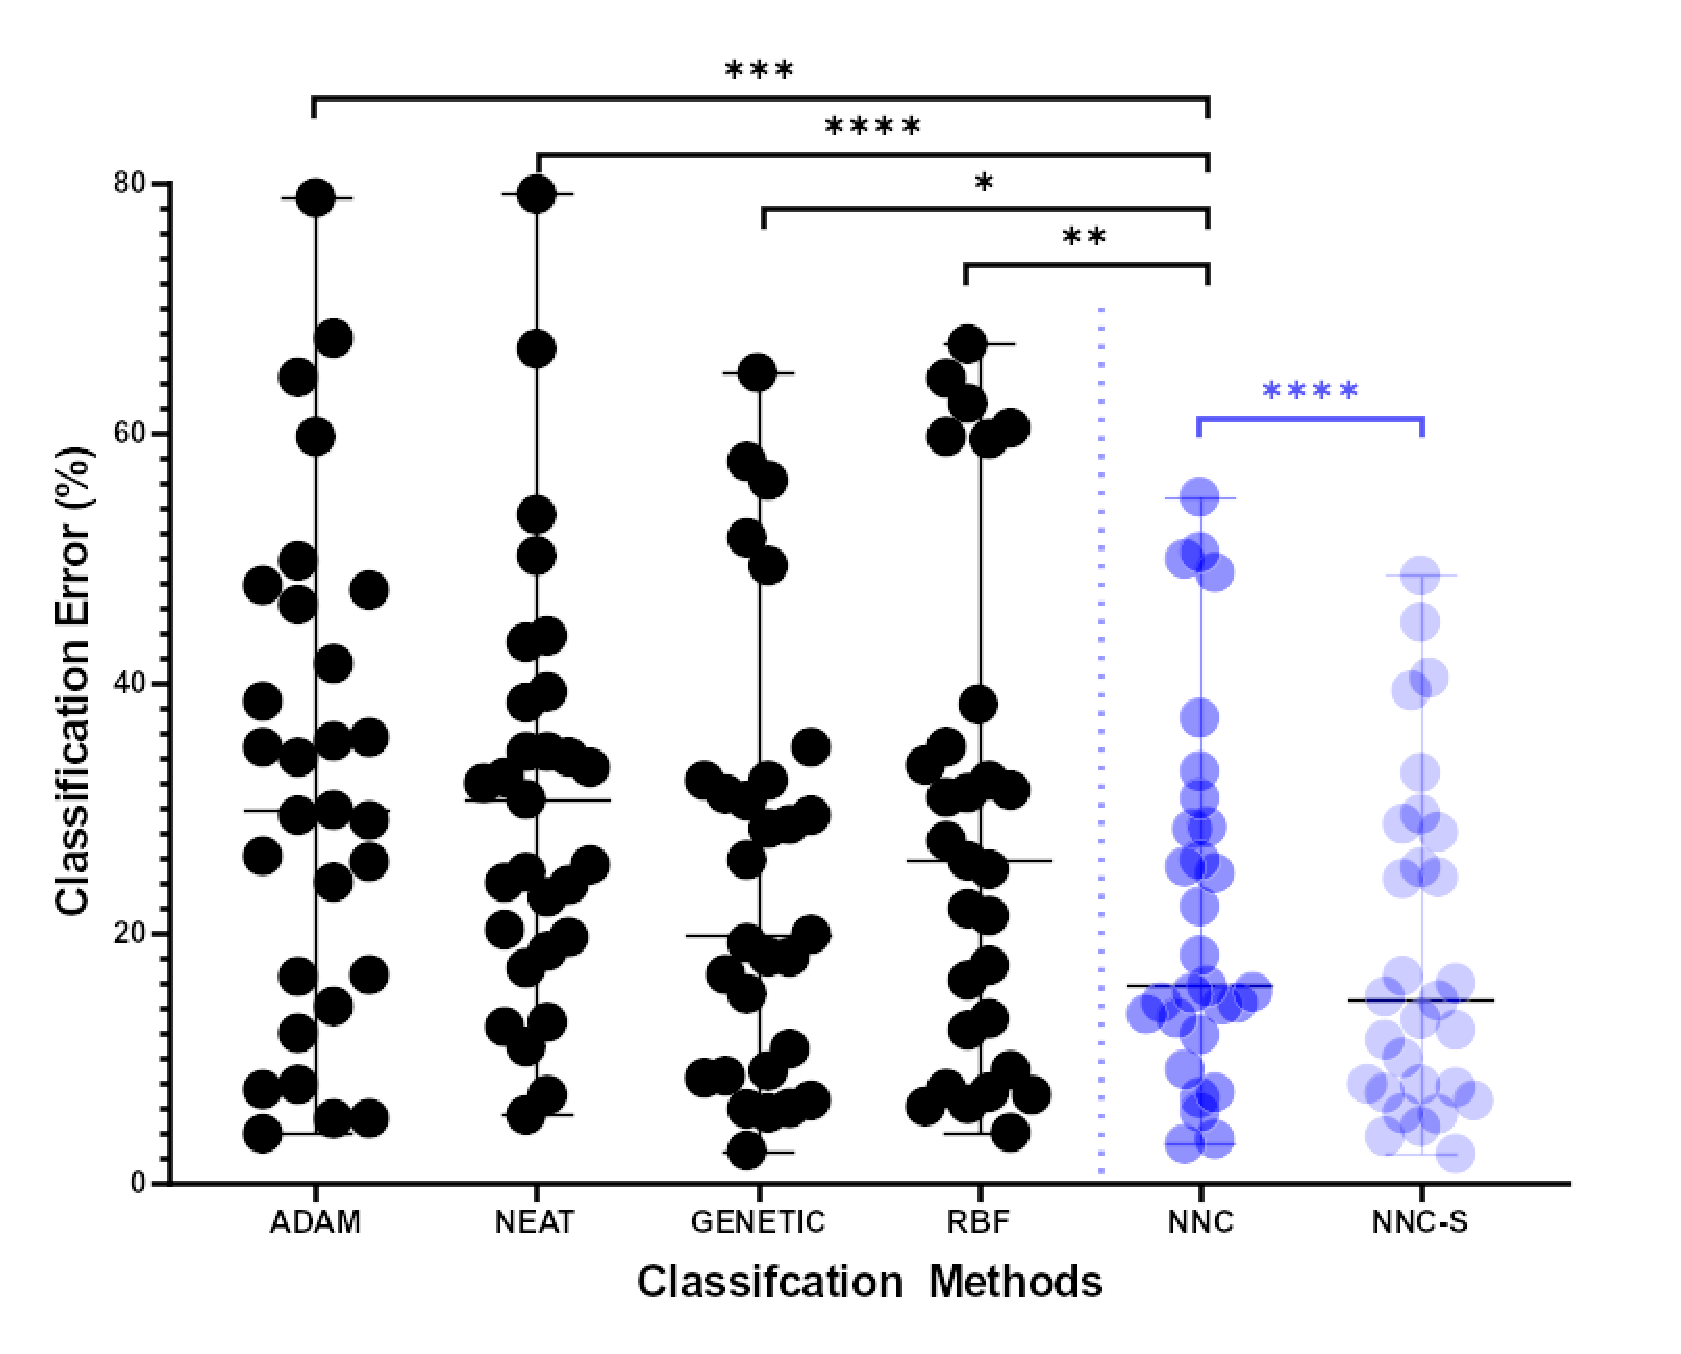
\includegraphics[scale=0.5]{gelocal_class}
\par\end{centering}
\caption{Scatter plot illustrating the variability and median classification
error rates for six machine learning algorithms, with statistical
significance denoted by asterisks. The NNC-S method demonstrates notably
lower error rates, as evidenced by the high statistical significance
relative to other methods, which may indicate its superior performance
in classification tasks.\label{fig:scatter_class}}

\end{figure}
Building on the previous analysis of classification methods, Figure
\ref{fig:scatter_regression} extends the evaluation to regression
algorithms, providing a comparative study of regression error rates
for the same six methods: ADAM, NEAT, GENETIC, RBF, NNC, and NNC-S.
Each data point reflects the regression error from a specific trial,
with the array of points for each method revealing the range of performance
outcomes. The median error rates are again represented by horizontal
lines across the clusters of dots, serving as a summary statistic
that facilitates a direct comparison of the methods' central performance
trends. The notation of statistical significance is consistent with
the previous figure, where asterisks convey the p-value levels, identifying
statistically meaningful differences in performance between the methods.

This plot reveals that the NNC-S method maintains its superior performance
in the context of regression tasks, demonstrating lower median regression
errors compared to the other methods. Significantly, it achieves a
markedly lower median regression error than its predecessor, NNC,
as indicated by the blue dots and supported by the three asterisks
({*}{*}{*}). This pattern of results underscores the broader applicability
of the NNC-S method's local optimization enhancements, not only in
classification accuracy but also in reducing regression errors.

\begin{figure}[H]
\begin{centering}
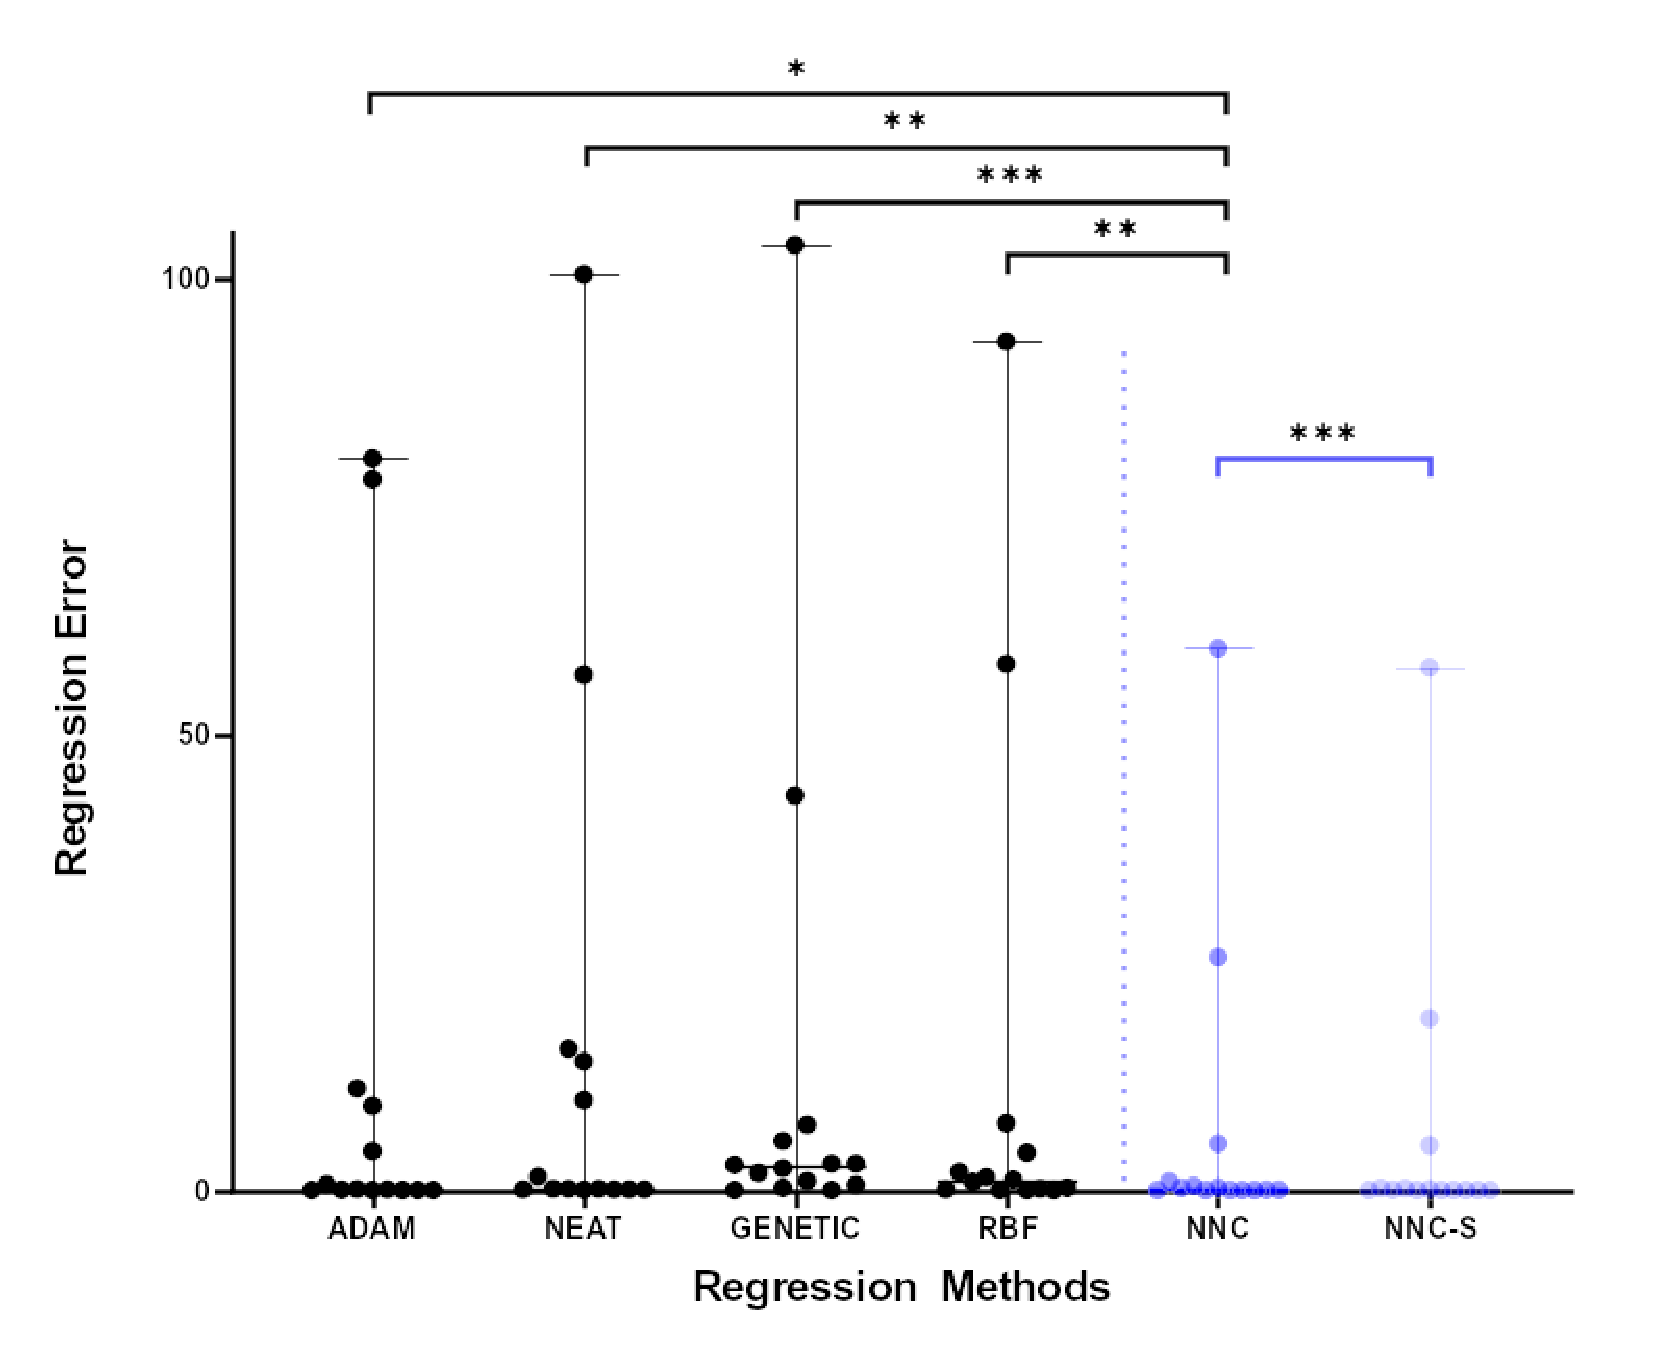
\includegraphics[scale=0.5]{gelocal_regression}
\par\end{centering}
\caption{Scatter plot of regression error rates for various regression methods,
demonstrating the distribution, median error rates, and statistical
significance of differences in performance. The NNC-S method, highlighted
in blue, shows statistically significant improvements in accuracy
over the NNC method, underlining the efficacy of local optimization
enhancements in regression tasks.\label{fig:scatter_regression}}

\end{figure}

Additionally, the effectiveness and the robustness of the proposed
method was evaluated by performing additional experiments with different
values for the critical parameter $g$ of the suggested Simulated
Annealing variant. This parameter is used to control the number of
random changes performed on any given chromosome. The experimental
results in the classification datasets are shown in Table \ref{tab:g_experiments}.
Clearly, no significant variation in the performance of the proposed
technique occurs when this critical parameter is varied.

\begin{table}[H]
\caption{Experiments with the parameter $g$ used in the modified Simulated
Annealing method. \label{tab:g_experiments}}

\centering{}%
\begin{tabular}{|c|c|c|c|c|}
\hline 
\textbf{DATASET} & \textbf{NNC-S($g=2)$} & \textbf{NNC-S($g=5)$} & \textbf{NNC-S($g=10$)} & \textbf{NNC-S($g=20)$}\tabularnewline
\hline 
\hline 
APPENDICITIS & 14.90\% & 15.00\% & 14.60\% & 14.50\%\tabularnewline
\hline 
AUSTRALIAN & 14.59\% & 14.85\% & 14.90\% & 15.04\%\tabularnewline
\hline 
BALANCE & 8.53\% & 7.68\% & 7.66\% & 7.56\%\tabularnewline
\hline 
CIRCULAR & 10.49\% & 8.81\% & 7.88\% & 7.50\%\tabularnewline
\hline 
CLEVELAND & 48.41\% & 48.31\% & 48.59\% & 48.10\%\tabularnewline
\hline 
DERMATOLOGY & 15.09\% & 13.80\% & 13.11\% & 13.29\%\tabularnewline
\hline 
ECOLI & 45.30\% & 45.12\% & 44.88\% & 44.36\%\tabularnewline
\hline 
HABERMAN & 27.80\% & 27.97\% & 28.73\% & 27.83\%\tabularnewline
\hline 
HAYES ROTH & 29.85\% & 28.85\% & 28.08\% & 29.15\%\tabularnewline
\hline 
HEART & 16.11\% & 15.04\% & 16.00\% & 14.78\%\tabularnewline
\hline 
HOUSEVOTES & 3.70\% & 4.22\% & 3.74\% & 3.70\%\tabularnewline
\hline 
IONOSPHERE & 10.54\% & 10.09\% & 10.03\% & 10.00\%\tabularnewline
\hline 
LIVERDISORDER & 31.41\% & 33.15\% & 32.82\% & 33.29\%\tabularnewline
\hline 
MAMMOGRAPHIC & 17.16\% & 17.25\% & 16.58\% & 16.99\%\tabularnewline
\hline 
PARKINSONS & 12.32\% & 12.89\% & 12.26\% & 12.11\%\tabularnewline
\hline 
PIMA & 26.12\% & 25.96\% & 25.26\% & 25.92\%\tabularnewline
\hline 
POPFAILURES & 5.58\% & 6.00\% & 5.52\% & 5.68\%\tabularnewline
\hline 
REGIONS2 & 24.71\% & 24.05\% & 24.47\% & 24.66\%\tabularnewline
\hline 
SAHEART & 30.04\% & 29.67\% & 29.52\% & 29.07\%\tabularnewline
\hline 
SEGMENT & 46.94\% & 42.37\% & 39.38\% & 41.19\%\tabularnewline
\hline 
STUDENT & 4.60\% & 4.73\% & 4.52\% & 4.48\%\tabularnewline
\hline 
TRANSFUSION & 24.28\% & 24.34\% & 24.33\% & 24.03\%\tabularnewline
\hline 
WDBC & 6.23\% & 6.22\% & 5.59\% & 5.68\%\tabularnewline
\hline 
WINE & 12.59\% & 11.30\% & 11.47\% & 9.24\%\tabularnewline
\hline 
Z\_F\_S & 9.57\% & 9.60\% & 7.93\% & 8.10\%\tabularnewline
\hline 
Z\_O\_N\_F\_S & 46.04\% & 43.36\% & 40.42\% & 41.54\%\tabularnewline
\hline 
ZO\_NF\_S & 9.69\% & 8.54\% & 6.60\% & 6.44\%\tabularnewline
\hline 
ZONF\_S & 2.58\% & 2.28\% & 2.36\% & 2.36\%\tabularnewline
\hline 
ZOO & 6.90\% & 7.00\% & 7.20\% & 7.70\%\tabularnewline
\hline 
\textbf{AVERAGE} & \textbf{19.38\%} & \textbf{18.91\%} & \textbf{18.43\%} & \textbf{18.42\%}\tabularnewline
\hline 
\end{tabular}
\end{table}
Continuing from the previous analysis, Figure \ref{fig:scatter_g}
presents the classification error rates for variations of the NNC-S
algorithm with differing values of the parameter $g$. The plot aims
to evaluate whether changes in the parameter $g$ led to statistically
significant differences in the algorithm's classification performance.
The horizontal bars on the plot indicate the median classification
error for each variation of the NNC-S method, providing a clear comparison
across the different parameter values. The statistical annotations
(\textquotedbl ns\textquotedbl{} for not significant, \textquotedbl{*}{*}”
for p \textless{} 0.01, and \textquotedbl{*}{*}{*}\textquotedbl{}
for p \textless{} 0.001) are used to denote the statistical significance
of the differences between the groups. It appears that some variations,
particularly between NNC-S (g=2) and NNC-S (g=5), as well as between
NNC-S (g=10) and NNC-S (g=20), do not show significant differences
in performance (denoted by \textquotedbl ns\textquotedbl ). In contrast,
other comparisons do reveal significant differences, suggesting that
certain values of g can indeed impact the classification error rates
of the NNC-S algorithm.

\begin{figure}[H]
\begin{centering}
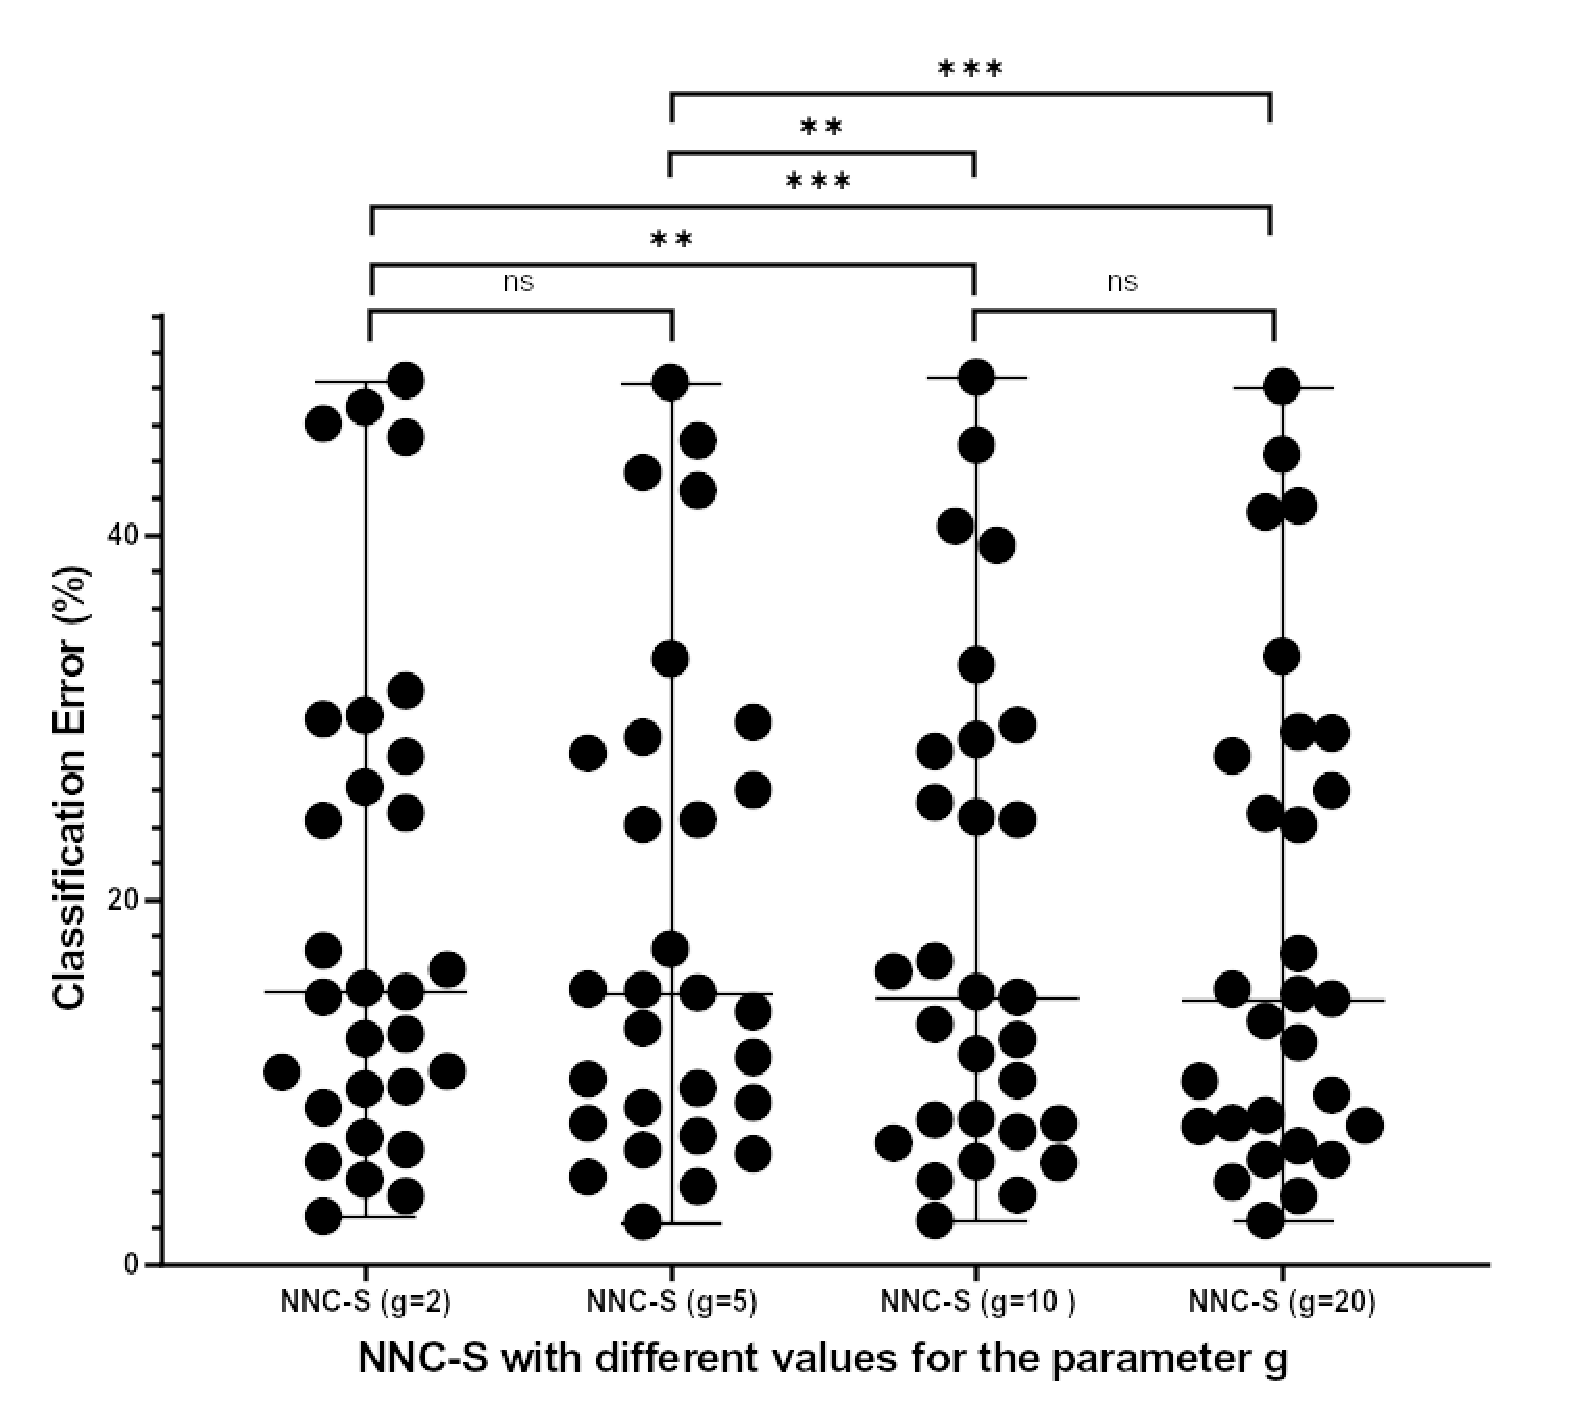
\includegraphics[scale=0.5]{gelocal_g}
\par\end{centering}
\caption{his figure examines the impact of varying the parameter g on the NNC-S
algorithm's classification errors, revealing that while some parameter
adjustments do not significantly affect performance, others result
in noticeable differences, as indicated by the statistical significance
annotations.\label{fig:scatter_g}}

\end{figure}

Furthermore, another experiment was executed by varying the parameter
$R$ of the proposed Simulated Annealing variant. This parameter controls
the range of changes performed in any given chromosome. The results
for this experiment are shown in Table \ref{tab:r_exper}. And this
time the method appeared quite robust in its performance, without
large variations in the error as measured in the test set. 

\begin{table}[H]
\caption{Experiments with the parameter $R$ of the modified Simulated Annealing
algorithm. The parameter $g$ was set to 10.\label{tab:r_exper}}

\centering{}%
\begin{tabular}{|c|c|c|c|c|}
\hline 
\textbf{DATASET} & \textbf{NNC-S($R=2)$} & \textbf{NNC-S($R=5)$} & \textbf{NNC-S($R=10$)} & \textbf{NNC-S($R=20)$}\tabularnewline
\hline 
\hline 
APPENDICITIS & 14.40\% & 14.90\% & 14.60\% & 15.20\%\tabularnewline
\hline 
AUSTRALIAN & 14.77\% & 14.78\% & 14.90\% & 14.70\%\tabularnewline
\hline 
BALANCE & 7.66\% & 7.74\% & 7.66\% & 7.66\%\tabularnewline
\hline 
CIRCULAR & 8.39\% & 8.29\% & 7.88\% & 7.78\%\tabularnewline
\hline 
CLEVELAND & 49.45\% & 49.28\% & 48.59\% & 47.11\%\tabularnewline
\hline 
DERMATOLOGY & 14.09\% & 12.54\% & 13.11\% & 11.34\%\tabularnewline
\hline 
ECOLI & 44.24\% & 46.30\% & 44.88\% & 44.48\%\tabularnewline
\hline 
HABERMAN & 27.33\% & 28.10\% & 28.73\% & 28.04\%\tabularnewline
\hline 
HAYES ROTH & 29.15\% & 27.92\% & 28.08\% & 26.46\%\tabularnewline
\hline 
HEART & 15.67\% & 15.52\% & 16.00\% & 15.15\%\tabularnewline
\hline 
HOUSEVOTES & 4.00\% & 3.62\% & 3.74\% & 4.52\%\tabularnewline
\hline 
IONOSPHERE & 10.14\% & 10.03\% & 10.03\% & 10.71\%\tabularnewline
\hline 
LIVERDISORDER & 32.80\% & 32.12\% & 32.82\% & 32.29\%\tabularnewline
\hline 
MAMMOGRAPHIC & 17.18\% & 16.78\% & 16.58\% & 16.62\%\tabularnewline
\hline 
PARKINSONS & 12.68\% & 12.16\% & 12.26\% & 11.95\%\tabularnewline
\hline 
PIMA & 25.72\% & 25.11\% & 25.26\% & 26.33\%\tabularnewline
\hline 
POPFAILURES & 5.87\% & 5.72\% & 5.52\% & 5.58\%\tabularnewline
\hline 
REGIONS2 & 23.55\% & 24.04\% & 24.47\% & 24.08\%\tabularnewline
\hline 
SAHEART & 29.48\% & 28.96\% & 29.52\% & 29.24\%\tabularnewline
\hline 
SEGMENT & 40.32\% & 40.23\% & 39.38\% & 40.82\%\tabularnewline
\hline 
STUDENT & 4.18\% & 4.50\% & 4.52\% & 4.78\%\tabularnewline
\hline 
TRANSFUSION & 24.60\% & 24.12\% & 24.33\% & 24.36\%\tabularnewline
\hline 
WDBC & 6.09\% & 5.68\% & 5.59\% & 5.46\%\tabularnewline
\hline 
WINE & 11.00\% & 10.30\% & 11.47\% & 9.41\%\tabularnewline
\hline 
Z\_F\_S & 8.33\% & 8.30\% & 7.93\% & 8.50\%\tabularnewline
\hline 
Z\_O\_N\_F\_S & 41.70\% & 43.42\% & 40.42\% & 41.44\%\tabularnewline
\hline 
ZO\_NF\_S & 7.58\% & 7.72\% & 6.60\% & 7.10\%\tabularnewline
\hline 
ZONF\_S & 2.50\% & 2.54\% & 2.36\% & 3.00\%\tabularnewline
\hline 
ZOO & 6.80\% & 6.30\% & 7.20\% & 6.10\%\tabularnewline
\hline 
\textbf{AVERAGE} & \textbf{18.61\%} & \textbf{18.52\%} & \textbf{18.43\%} & \textbf{18.28\%}\tabularnewline
\hline 
\end{tabular}
\end{table}


\section{Conclusions\label{sec:Conclusions}}

In the current work, an extension of the original Grammatical Evolution
has been proposed, which was applied in the Neural Construction method.
In this extension, an application of a modified optimization method
was suggested, in order to improve the efficiency of the underlying
technique. The proposed optimization algorithm was a variant of the
Simulated Annealing method, that was applied on a series of chromosomes,
that was randomly from the Grammatical Evolution procedure. This method
was chosen because of its widespread use in many applications but
because of its ability to handle integer representations, since the
chromosomes in Grammatical Evolution are vectors of integers. Of course,
other local optimization techniques could be incorporated, such as
tabu search \citep{tabu} or hill climbing \citep{hill} as feature
extensions of the proposed method.

The proposed modification was applied to the Neural Network Construction
method and its efficiency was measured on some classification and
regression datasets commonly used. Based on the experimental results,
it has become clear that the proposed variant significantly improves
the performance of the technique both on classification datasets and
on data fitting datasets. Also, the effectiveness and the robustness
of the proposed modification were measured using experiments with
different values of some critical parameters of the current Simulated
Annealing variant. These experiments indicated that the method tends
to be rubost, since the experimental results does not depend on the
selection of any critical parameter of the Simulated Annealing variant.

Future work may include application of the local search procedure
in other Grammatical Evolution applications, such as feature construction,
creation of classification rules etc. Also, the proposed process can
be significantly accelerated by the use of parallel optimization techniques
\citep{psa}, which take advantage of modern computational structures.

\vspace{6pt}


\authorcontributions{I.G.T., A.T. and E.K. conceived the idea and methodology and supervised
the technical part regarding the software. I.G.T. conducted the experiments,
employing several datasets, and provided the comparative experiments.
A.T. performed the statistical analysis. E.K. and all other authors
prepared the manuscript. E.K. and I.G.T. organized the research team
and A.T. supervised the project. All authors have read and agreed
to the published version of the manuscript.}

\funding{This research received no external funding.}

\institutionalreview{Not applicable.}

\informedconsent{Not applicable.}

\acknowledgments{This research has been financed by the European Union : Next Generation
EU through the Program Greece 2.0 National Recovery and Resilience
Plan , under the call RESEARCH -- CREATE -- INNOVATE, project name
“iCREW: Intelligent small craft simulator for advanced crew training
using Virtual Reality techniques\textquotedbl{} (project code:TAEDK-06195}

\conflictsofinterest{The authors declare no conflict of interest.}

\appendixtitles{no}

\appendixstart{}

\appendix

\begin{adjustwidth}{-\extralength}{0cm}{}

\reftitle{References}
\begin{thebibliography}{99}
\bibitem{ec_review}N. Yusup, A. M. Zain, S. Z. M. Hashim, Evolutionary
techniques in optimizing machining parameters: Review and recent applications
(2007--2011), Expert Systems with Applications \textbf{39.10}, pp.
9909-9927, 2012.

\bibitem{Holland1}J.H. Holland, Genetic algorithms. Scientific american
\textbf{267}, pp. 66-73, 1992.

\bibitem{Stender}J. Stender, Parallel Genetic Algorithms:Theory \&
Applications. Edition: IOS Press, 1993. 

\bibitem{genetic1}D. Goldberg, Genetic Algorithms in Search, Optimization
and Machine Learning, Addison-Wesley Publishing Company, Reading,
Massachussets, 1989.

\bibitem{genetic2}Z. Michaelewicz, Genetic Algorithms + Data Structures
= Evolution Programs. Springer - Verlag, Berlin, 1996.

\bibitem{ge1}M. O’Neill, C. Ryan, Grammatical evolution, IEEE Trans.
Evol. Comput. \textbf{5,}pp. 349--358, 2001.

\bibitem{bnf1}J. W. Backus. The Syntax and Semantics of the Proposed
International Algebraic Language of the Zurich ACM-GAMM Conference.
Proceedings of the International Conference on Information Processing,
UNESCO, 1959, pp.125-132.

\bibitem{ge_program1}C. Ryan, J. Collins, M. O’Neill, Grammatical
evolution: Evolving programs for an arbitrary language. In: Banzhaf,
W., Poli, R., Schoenauer, M., Fogarty, T.C. (eds) Genetic Programming.
EuroGP 1998. Lecture Notes in Computer Science, vol 1391. Springer,
Berlin, Heidelberg, 1998.

\bibitem{ge_program2}M. O’Neill, M., C. Ryan, Evolving Multi-line
Compilable C Programs. In: Poli, R., Nordin, P., Langdon, W.B., Fogarty,
T.C. (eds) Genetic Programming. EuroGP 1999. Lecture Notes in Computer
Science, vol 1598. Springer, Berlin, Heidelberg, 1999.

\bibitem{ge_credit}A. Brabazon, M. O'Neill, Credit classification
using grammatical evolution, Informatica \textbf{30.3}, 2006.

\bibitem{ge_intrusion}S. Şen, J.A. Clark. A grammatical evolution
approach to intrusion detection on mobile ad hoc networks, In: Proceedings
of the second ACM conference on Wireless network security, 2009.

\bibitem{ge_water}L. Chen, C.H. Tan, S.J. Kao, T.S. Wang, Improvement
of remote monitoring on water quality in a subtropical reservoir by
incorporating grammatical evolution with parallel genetic algorithms
into satellite imagery, Water Research \textbf{ 42}, pp. 296-306,
2008.

\bibitem{ge_glykemia}J. I. Hidalgo, J. M. Colmenar, J.L. Risco-Martin,
A. Cuesta-Infante, E. Maqueda, M. Botella,J. A. Rubio, Modeling glycemia
in humans by means of Grammatical Evolution, Applied Soft Computing
\textbf{20}, pp. 40-53, 2014.

\bibitem{ge_ant}J. Tavares, F.B. Pereira, Automatic Design of Ant
Algorithms with Grammatical Evolution. In: Moraglio, A., Silva, S.,
Krawiec, K., Machado, P., Cotta, C. (eds) Genetic Programming. EuroGP
2012. Lecture Notes in Computer Science, vol 7244. Springer, Berlin,
Heidelberg, 2012.

\bibitem{ge_datacenter}M. Zapater, J.L. Risco-Martín, P. Arroba,
J.L. Ayala, J.M. Moya, R. Hermida, Runtime data center temperature
prediction using Grammatical Evolution techniques, Applied Soft Computing
\textbf{49}, pp. 94-107, 2016.

\bibitem{ge_trig}C. Ryan, M. O’Neill, J.J. Collins, Grammatical evolution:
Solving trigonometric identities, proceedings of Mendel. Vol. 98.
1998.

\bibitem{ge_music}A.O. Puente, R. S. Alfonso, M. A. Moreno, Automatic
composition of music by means of grammatical evolution, In: APL '02:
Proceedings of the 2002 conference on APL: array processing languages:
lore, problems, and applications July 2002 Pages 148--155. 

\bibitem{ge_nn}Lídio Mauro Limade Campo, R. Célio Limã Oliveira,Mauro
Roisenberg, Optimization of neural networks through grammatical evolution
and a genetic algorithm, Expert Systems with Applications \textbf{56},
pp. 368-384, 2016.

\bibitem{ge_nn2}K. Soltanian, A. Ebnenasir, M. Afsharchi, Modular
Grammatical Evolution for the Generation of Artificial Neural Networks,
Evolutionary Computation \textbf{30}, pp 291--327, 2022.

\bibitem{ge_constant}I. Dempsey, M.O' Neill, A. Brabazon, Constant
creation in grammatical evolution, International Journal of Innovative
Computing and Applications \textbf{1} , pp 23--38, 2007.

\bibitem{ge_pacman}E. Galván-López, J.M. Swafford, M. O’Neill, A.
Brabazon, Evolving a Ms. PacMan Controller Using Grammatical Evolution.
In: , et al. Applications of Evolutionary Computation. EvoApplications
2010. Lecture Notes in Computer Science, vol 6024. Springer, Berlin,
Heidelberg, 2010.

\bibitem{ge_supermario}N. Shaker, M. Nicolau, G. N. Yannakakis, J.
Togelius, M. O'Neill, Evolving levels for Super Mario Bros using grammatical
evolution, 2012 IEEE Conference on Computational Intelligence and
Games (CIG), 2012, pp. 304-31.

\bibitem{ge_energy}D. Martínez-Rodríguez, J. M. Colmenar, J. I. Hidalgo,
R.J. Villanueva Micó, S. Salcedo-Sanz, Particle swarm grammatical
evolution for energy demand estimation, Energy Science and Engineering
\textbf{8}, pp. 1068-1079, 2020.

\bibitem{ge_comb}N. R. Sabar, M. Ayob, G. Kendall, R. Qu, Grammatical
Evolution Hyper-Heuristic for Combinatorial Optimization Problems,
IEEE Transactions on Evolutionary Computation \textbf{17}, pp. 840-861,
2013.

\bibitem{ge_crypt}C. Ryan, M. Kshirsagar, G. Vaidya, G. et al. Design
of a cryptographically secure pseudo random number generator with
grammatical evolution. Sci Rep \textbf{12}, 8602, 2022.

\bibitem{ge_decision}P.J. Pereira, P. Cortez, R. Mendes, Multi-objective
Grammatical Evolution of Decision Trees for Mobile Marketing user
conversion prediction, Expert Systems with Applications \textbf{168},
114287, 2021.

\bibitem{ge_analog}F. Castejón, E.J. Carmona, Automatic design of
analog electronic circuits using grammatical evolution, Applied Soft
Computing \textbf{62}, pp. 1003-1018, 2018.

\bibitem{ge_structured1}N. Lourenço, F.B. Pereira, E, Costa, Unveiling
the properties of structured grammatical evolution, Genetic Programming
and Evolvable Machines \textbf{17} , pp. 251-289, 2016.

\bibitem{ge_structured2}N. Lourenço, F. Assunção, F.B. Pereira, E.
Costa, P. Machado, Structured grammatical evolution: a dynamic approach,
Handbook of grammatical evolution, pp. 137-161, 2018.

\bibitem{pge}M. O’Neill, A. Brabazon, M. Nicolau, S.M. Garraghy,
P. Keenan, $\pi$Grammatical Evolution. In: Deb, K. (eds) Genetic
and Evolutionary Computation -- GECCO 2004. GECCO 2004. Lecture Notes
in Computer Science, vol 3103. Springer, Berlin, Heidelberg, 2004.

\bibitem{pso1}Riccardo Poli, James Kennedy kennedy, Tim Blackwell,
Particle swarm optimization An Overview, Swarm Intelligence \textbf{1},
pp 33-57, 2007. 

\bibitem{ge_swarm1}M. O’Neill, A. Brabazon, Grammatical swarm: The
generation of programs by social programming. Natural Computing \textbf{5},
pp. 443-462, 2006.

\bibitem{ge_swarm2}E. Ferrante, E. Duéñez-Guzmán, A.E. Turgut, T.
Wenseleers, GESwarm: Grammatical evolution for the automatic synthesis
of collective behaviors in swarm robotics. In Proceedings of the 15th
annual conference on Genetic and evolutionary computation, pp. 17-24,
2013.

\bibitem{probge}J. Mégane, N. Lourenço, P. Machado, Probabilistic
Grammatical Evolution. In: Hu, T., Lourenço, N., Medvet, E. (eds)
Genetic Programming. EuroGP 2021. Lecture Notes in Computer Science,
vol 12691. Springer, Cham, 2021.

\bibitem{ge_par1}O. Popelka, P. Osmera, Parallel Grammatical Evolution
for Circuit Optimization. In: Hornby, G.S., Sekanina, L., Haddow,
P.C. (eds) Evolvable Systems: From Biology to Hardware. ICES 2008.
Lecture Notes in Computer Science, vol 5216. Springer, Berlin, Heidelberg.
https://doi.org/10.1007/978-3-540-85857-7\_40

\bibitem{ge_par2}P. Ošmera, Two level parallel grammatical evolution,
Advances in Computational Algorithms and Data Analysis pp. 509-525,
2009.

\bibitem{ge_geva}M. O'Neill, E. Hemberg, C. Gilligan, E. Bartley,
J. McDermott, A. Brabazon, GEVA: grammatical evolution in Java. ACM
SIGEVOlution \textbf{3}, pp. 17-22, 2008.

\bibitem{ge_christiansen}A. Ortega, M. de la Cruz, M. Alfonseca,
Christiansen Grammar Evolution: Grammatical Evolution With Semantics,
IEEE Transactions on Evolutionary Computation \textbf{11}, pp. 77-90,
Feb. 2007.

\bibitem{ge_gramevol}F. Noorian, A.M. de Silva, P.H.W. Leong, gramEvol:
Grammatical Evolution in R, Journal of Statistical Software \textbf{71},
pp. 1--26, 2016.

\bibitem{ge_gelab}M.A. Raja, C. Ryan, GELAB - A Matlab Toolbox for
Grammatical Evolution. In: Yin, H., Camacho, D., Novais, P., Tallón-Ballesteros,
A. (eds) Intelligent Data Engineering and Automated Learning -- IDEAL
2018. IDEAL 2018. Lecture Notes in Computer Science(), vol 11315,
2018. Springer, Cham. https://doi.org/10.1007/978-3-030-03496-2\_22

\bibitem{ge_genclass}N.Anastasopoulos, I.G. Tsoulos, A. Tzallas,
GenClass: A parallel tool for data classification based on Grammatical
Evolution, SoftwareX \textbf{16}, 100830, 2021.

\bibitem{ge_qfc}I.G. Tsoulos, QFC: A Parallel Software Tool for Feature
Construction, Based on Grammatical Evolution, Algorithms \textbf{15},
295, 2022.

\bibitem{ge_local1}S. Yang, S. N. Jat, Genetic Algorithms With Guided
and Local Search Strategies for University Course Timetabling, IEEE
Transactions on Systems, Man, and Cybernetics, Part C (Applications
and Reviews) \textbf{41}, pp. 93-106, 2011.

\bibitem{ge_local2}M. Sivaram, K. Batri, A.S. Mohammed, V. Porkodi,
Exploiting the Local Optima in Genetic Algorithm using Tabu Search.
Indian Journal of Science and Technology \textbf{12}, pp. 1--13,
2019.

\bibitem{bfgs}Y.H. Dai, Convergence Properties of the BFGS Algoritm,
SIAM Journal on Optimization \textbf{13}, pp. 693-701, 2002.

\bibitem{siman_main}S. Kirkpatrick, C.D. Gelatt Jr, M.P. Vecchi,
Optimization by simulated annealing, Science \textbf{220}, pp. 671-680,
1983.

\bibitem{siman_image}M.C. Robini, T. Rastello, I.E. Magnin, Simulated
annealing, acceleration techniques, and image restoration, IEEE Transactions
on Image processing \textbf{8.10}, pp. 1374-1387, 1999.

\bibitem{siman_protein}L. Zhang, H. Ma, W. Qian, H. Li, Protein structure
optimization using improved simulated annealing algorithm on a three-dimensional
AB off-lattice model. Computational Biology and Chemistry \textbf{85},
107237, 2020.

\bibitem{siman_resource}J.C.J. H. Aerts, G.B.M. Heuvelink, Using
simulated annealing for resource allocation, International Journal
of Geographical Information Science \textbf{16}, pp. 571-587, 2002.

\bibitem{siman_convex}A.T. Kalai, S. Vempala, Simulated annealing
for convex optimization, Mathematics of Operations Research \textbf{31.2},
pp. 253-266, 2006.

\bibitem{siman_deep}L.M. Rasdi Rere, M.I. Fanany, A. M. Arymurthy,
Simulated Annealing Algorithm for Deep Learning, Procedia Computer
Science \textbf{72}, pp. 137-144, 2015.

\bibitem{nnc_tsoulos}I.G. Tsoulos, D. Gavrilis, E. Glavas, Neural
network construction and training using grammatical evolution. Neurocomputing
\textbf{72}, pp. 269-277, 2008.

\bibitem{UCL}M. Kelly, R. Longjohn, K. Nottingham, The UCI Machine
Learning Repository. 2023. Available online: https://archive.ics.uci.edu
(accessed on 18 February 2024).

\bibitem{Keel}J. Alcalá-Fdez, A. Fernandez, J. Luengo, J. Derrac,
S. García, L. Sánchez, F. Herrera. KEEL Data-Mining Software Tool:
Data Set Repository, Integration of Algorithms and Experimental Analysis
Framework. Journal of Multiple-Valued Logic and Soft Computing 17,
pp. 255-287, 2011.

\bibitem{appendicitis}Weiss, Sholom M. and Kulikowski, Casimir A.,
Computer Systems That Learn: Classification and Prediction Methods
from Statistics, Neural Nets, Machine Learning, and Expert Systems,
Morgan Kaufmann Publishers Inc, 1991.

\bibitem{australian}J.R. Quinlan, Simplifying Decision Trees. International
Journal of Man-Machine Studies \textbf{27}, pp. 221-234, 1987. 

\bibitem{balance}T. Shultz, D. Mareschal, W. Schmidt, Modeling Cognitive
Development on Balance Scale Phenomena, Machine Learning \textbf{16},
pp. 59-88, 1994.

\bibitem{cleveland1}Z.H. Zhou,Y. Jiang, NeC4.5: neural ensemble based
C4.5,\textquotedbl{} in IEEE Transactions on Knowledge and Data Engineering
\textbf{16}, pp. 770-773, 2004.

\bibitem{cleveland2}R. Setiono , W.K. Leow, FERNN: An Algorithm for
Fast Extraction of Rules from Neural Networks, Applied Intelligence
\textbf{12}, pp. 15-25, 2000.

\bibitem{dermatology}G. Demiroz, H.A. Govenir, N. Ilter, Learning
Differential Diagnosis of Eryhemato-Squamous Diseases using Voting
Feature Intervals, Artificial Intelligence in Medicine. \textbf{13},
pp. 147--165, 1998.

\bibitem{ecoli}P. Horton, K.Nakai, A Probabilistic Classification
System for Predicting the Cellular Localization Sites of Proteins,
In: Proceedings of International Conference on Intelligent Systems
for Molecular Biology \textbf{4}, pp. 109-15, 1996.

\bibitem{heart}I. Kononenko, E. Šimec, M. Robnik-Šikonja, Overcoming
the Myopia of Inductive Learning Algorithms with RELIEFF, Applied
Intelligence \textbf{7}, pp. 39--55, 1997

\bibitem{hayesroth}B. Hayes-Roth, B., F. Hayes-Roth. Concept learning
and the recognition and classification of exemplars. Journal of Verbal
Learning and Verbal Behavior \textbf{16}, pp. 321-338, 1977.

\bibitem{housevotes}R.M. French, N. Chater, Using noise to compute
error surfaces in connectionist networks: a novel means of reducing
catastrophic forgetting, Neural Comput. \textbf{14}, pp. 1755-1769,
2002.

\bibitem{ion1}J.G. Dy , C.E. Brodley, Feature Selection for Unsupervised
Learning, The Journal of Machine Learning Research \textbf{5}, pp
845--889, 2004.

\bibitem{ion2}S. J. Perantonis, V. Virvilis, Input Feature Extraction
for Multilayered Perceptrons Using Supervised Principal Component
Analysis, Neural Processing Letters \textbf{10}, pp 243--252, 1999.

\bibitem{liver} J. Garcke, M. Griebel, Classification with sparse
grids using simplicial basis functions, Intell. Data Anal. \textbf{6},
pp. 483-502, 2002.

\bibitem{mammographic}M. Elter, R. Schulz-Wendtland, T. Wittenberg,
The prediction of breast cancer biopsy outcomes using two CAD approaches
that both emphasize an intelligible decision process, Med Phys. \textbf{34},
pp. 4164-72, 2007.

\bibitem{parkinsons}M.A. Little, P.E. McSharry, E.J. Hunter, J. Spielman,
L.O. Ramig, Suitability of dysphonia measurements for telemonitoring
of Parkinson's disease. IEEE Trans Biomed Eng. \textbf{56}, pp. 1015-1022,
2009.

\bibitem{pima}J.W. Smith, J.E. Everhart, W.C. Dickson, W.C. Knowler,
R.S. Johannes, Using the ADAP learning algorithm to forecast the onset
of diabetes mellitus, In: Proceedings of the Symposium on Computer
Applications and Medical Care IEEE Computer Society Press, pp.261-265,
1988.

\bibitem{popfailures}D.D. Lucas, R. Klein, J. Tannahill, D. Ivanova,
S. Brandon, D. Domyancic, Y. Zhang, Failure analysis of parameter-induced
simulation crashes in climate models, Geoscientific Model Development
\textbf{6}, pp. 1157-1171, 2013.

\bibitem{regions}N. Giannakeas, M.G. Tsipouras, A.T. Tzallas, K.
Kyriakidi, Z.E. Tsianou, P. Manousou, A. Hall, E.C. Karvounis, V.
Tsianos, E. Tsianos, A clustering based method for collagen proportional
area extraction in liver biopsy images (2015) Proceedings of the Annual
International Conference of the IEEE Engineering in Medicine and Biology
Society, EMBS, 2015-November, art. no. 7319047, pp. 3097-3100. 

\bibitem{saheart}T. Hastie, R. Tibshirani, Non-parametric logistic
and proportional odds regression, JRSS-C (Applied Statistics) \textbf{36},
pp. 260--276, 1987.

\bibitem{segment}M. Dash, H. Liu, P. Scheuermann, K. L. Tan, Fast
hierarchical clustering and its validation, Data \& Knowledge Engineering
\textbf{44}, pp 109--138, 2003.

\bibitem{student}P. Cortez, A. M. Gonçalves Silva, Using data mining
to predict secondary school student performance, In Proceedings of
5th FUture BUsiness TEChnology Conference (FUBUTEC 2008) (pp. 5--12).
EUROSIS-ETI, 2008.

\bibitem{transfusion}I-Cheng Yeh, King-Jang Yang, Tao-Ming Ting,
Knowledge discovery on RFM model using Bernoulli sequence, Expert
Systems with Applications \textbf{36}, pp. 5866-5871, 2009.

\bibitem{wdbc}W.H. Wolberg, O.L. Mangasarian, Multisurface method
of pattern separation for medical diagnosis applied to breast cytology,
Proc Natl Acad Sci U S A. \textbf{87}, pp. 9193--9196, 1990.

\bibitem{wine1}M. Raymer, T.E. Doom, L.A. Kuhn, W.F. Punch, Knowledge
discovery in medical and biological datasets using a hybrid Bayes
classifier/evolutionary algorithm. IEEE transactions on systems, man,
and cybernetics. Part B, Cybernetics : a publication of the IEEE Systems,
Man, and Cybernetics Society, \textbf{33} , pp. 802-813, 2003.

\bibitem{wine2}P. Zhong, M. Fukushima, Regularized nonsmooth Newton
method for multi-class support vector machines, Optimization Methods
and Software \textbf{22}, pp. 225-236, 2007.

\bibitem{eeg}R.G. Andrzejak, K. Lehnertz, F. Mormann, C. Rieke, P.
David, and C. E. Elger, Indications of nonlinear deterministic and
finite-dimensional structures in time series of brain electrical activity:
Dependence on recording region and brain state, Phys. Rev. E \textbf{64},
pp. 1-8, 2001.

\bibitem{zoo}M. Koivisto, K. Sood, Exact Bayesian Structure Discovery
in Bayesian Networks, The Journal of Machine Learning Research\textbf{
5}, pp. 549--573, 2004.

\bibitem{abalone}W. J Nash, T.L. Sellers, S.R. Talbot, A.J. Cawthor,
W.B. Ford, The Population Biology of Abalone (\_Haliotis\_ species)
in Tasmania. I. Blacklip Abalone (\_H. rubra\_) from the North Coast
and Islands of Bass Strait, Sea Fisheries Division, Technical Report
No. 48 (ISSN 1034-3288), 1994.

\bibitem{airfoil}T.F. Brooks, D.S. Pope, A.M. Marcolini, Airfoil
self-noise and prediction. Technical report, NASA RP-1218, July 1989. 

\bibitem{concrete}I.Cheng Yeh, Modeling of strength of high performance
concrete using artificial neural networks, Cement and Concrete Research.
\textbf{28}, pp. 1797-1808, 1998. 

\bibitem{key23}D. Harrison and D.L. Rubinfeld, Hedonic prices and
the demand for clean ai, J. Environ. Economics \& Management \textbf{5},
pp. 81-102, 1978.

\bibitem{Adam}D. P. Kingma, J. L. Ba, ADAM: a method for stochastic
optimization, in: Proceedings of the 3rd International Conference
on Learning Representations (ICLR 2015), pp. 1--15, 2015.

\bibitem{neat}K. O. Stanley, R. Miikkulainen, Evolving Neural Networks
through Augmenting Topologies, Evolutionary Computation \textbf{10},
pp. 99-127, 2002.

\bibitem{powell}M.J.D Powell, A Tolerant Algorithm for Linearly Constrained
Optimization Calculations, Mathematical Programming \textbf{45}, pp.
547-566, 1989. 

\bibitem{tabu}F. Glover, Parametric tabu-search for mixed integer
programs. Computers \& Operations Research \textbf{33}, pp. 2449-2494,
2006.

\bibitem{hill}A. Lim, B. Rodrigues, X. Zhang, A simulated annealing
and hill-climbing algorithm for the traveling tournament problem.
European Journal of Operational Research \textbf{174}, pp.1459-1478,
2006.

\bibitem{psa}A. Bevilacqua, A methodological approach to parallel
simulated annealing on an SMP system. Journal of Parallel and Distributed
Computing \textbf{62}, pp. 1548-1570, 2002.

\end{thebibliography}
%%%%%%%%%%%%%%%%%%%%%%%%%%%%%%%%%%%%%%%%%%
%% for journal Sci
%\reviewreports{\\
%Reviewer 1 comments and authors' response\\
%Reviewer 2 comments and authors' response\\
%Reviewer 3 comments and authors' response
%}
%%%%%%%%%%%%%%%%%%%%%%%%%%%%%%%%%%%%%%%%%%

\end{adjustwidth}{}
\end{document}
